\chapter{Schwarzschild black hole}
\label{s:sch}
\index{Schwarzschild!black hole}

\minitoc

\section{Introduction}

After having discussed stationary black holes in Chap.~\ref{s:sta},
we examine here the simplest of them: the Schwarzschild black hole.
Let us recall that the prime importance of this object
in general relativity stems from the no-hair theorem (Sec.~\ref{s:sta:no-hair}),
which implies that any non-rotating black hole in an asymptotically flat
4-dimensional spacetime must be a Schwarzschild black hole.

\section{The Schwarzschild-(anti-)de Sitter solution}

\subsection{Vacuum Einstein equation with a cosmological constant}

Let us search for a static and spherically symmetric solution of the
Einstein equation (\ref{e:bas:Einstein_eq}) in a vacuum
4-dimensional spacetime $(\M,\w{g})$ with some arbitrary cosmological constant
$\Lambda$. Setting $\w{T}=0$ in Eq.~(\ref{e:bas:Einstein_eq}) yields
the equation to solve:
\be \label{e:sch:vac_Einstein_eq}
     \w{R} + \left(\Lambda - \frac{1}{2}\, R\right) \w{g} = 0 ,
\ee
$\w{R}$ being the Ricci tensor of $\w{g}$ and $R:=g^{\mu\nu} R_{\mu\nu}$ its
trace with respect to $\w{g}$, i.e. the so-called Ricci scalar
(cf. Sec.~\ref{s:bas:Ricci_tensor} in Appendix~\ref{s:bas}).
Let us first note that Eq.~(\ref{e:sch:vac_Einstein_eq}) implies a
constraint on $R$. Indeed the trace of Eq.~(\ref{e:sch:vac_Einstein_eq})
with respect to $\w{g}$ is
\[
    R + \left(\Lambda - \frac{1}{2}\, R\right) \times 4 = 0 ,
\]
hence
\be \label{e:sch:R_4Lamb}
    \encadre{R = 4\Lambda} .
\ee
In particular $R$ is constant.
Inserting this value back into (\ref{e:sch:vac_Einstein_eq}), we get
\be \label{e:sch:vac_Einstein_eq_Lamb}
    \encadre{ \w{R} = \Lambda \, \w{g} } .
\ee
Since this equation yields (\ref{e:sch:R_4Lamb}) as well, we conclude
that it is equivalent to (\ref{e:sch:vac_Einstein_eq}).

\subsection{Static and spherically symmetric metric} \label{s:sch:static_spher}

Let us assume that the spacetime $(\M,\w{g})$ is \defin{static}\index{static spacetime}:
the translation group $(\R,+)$ is a isometry group of $(\M,\w{g})$
(cf. Sec.~\ref{s:neh:symmetries}), with orbits that are timelike
(stationarity property) and hypersurface-orthogonal (staticity property, cf. Sec.~\ref{s:sta:staticity_thm}). Let us denote by $\w{\xi}$ the associated Killing vector
field (unique up to some constant rescaling), i.e. the generator of the
isometry group $(\R,+)$ (cf. Sec.~\ref{s:neh:symmetries}).

We may foliate $\M$ by a 1-parameter family of hypersurfaces
$\left(\Sigma_t\right)_{t\in\R}$, such that $\w{\xi}$ is normal to
all $\Sigma_t$'s and $t$ is a parameter associated to $\w{\xi}$:
\be \label{e:sch:xi_t}
    \w{\xi}(t) = 1
\ee
or equivalently,
\[
    \langle \dd t , \w{\xi} \rangle = 1.
\]

In addition to being static, we assume that $(\M,\w{g})$ is \defin{spherically symmetric},
i.e. that it is invariant under the action of the rotation group $\mathrm{SO}(3)$,
whose orbits are spacelike 2-spheres (cf. Sec.~\ref{s:neh:symmetries}).
Let $\Sp$ be some generic orbit 2-sphere. The static Killing vector field $\w{\xi}$
must be orthogonal to $\Sp$, otherwise the orthogonal projection of $\w{\xi}$
onto $\Sp$ would define some privileged directions on $\Sp$, which is incompatible
with spherical symmetry. The orthogonality of $\w{\xi}$ and $\Sp$ implies
that $\Sp\subset\Sigma_t$. Let $(x^a)=(\th,\ph)$ be spherical coordinates on
$\Sp$. The (Riemannian) metric $\w{q}$ induced by $\w{g}$ on $\Sp$ is given by
\be
    q_{ab}\, \D x^a\, \D x^b = r^2 \left( \D\th^2 + \sin^2\th\, \D\ph^2 \right) .
\ee
The positive coefficient $r^2$ in front of the standard spherical element must be
constant over $\Sp$, by virtue of spherical symmetry. The area of $\Sp$ is
then $A=4\pi r^2$. For this reason, $r$ is called the \defin{areal radius}\index{areal!radius}
of $\Sp$. Letting $\Sp$ vary, $r$ can be considered as a scalar field on
$\M$. If $\dd r \not = 0$, we may use it a coordinate. Since $\Sp\subset \Sigma_t$,
$(r,\th,\ph)$ is a coordinate system on each hypersurface $\Sigma_t$.
The set $(t,r,\th,\ph)$,
where $t$ is adapted to $\w{\xi}$ thanks to (\ref{e:sch:xi_t}), is then a
spacetime coordinate system and, by construction, the expression of the metric tensor
with respect to this system is
\be \label{e:sch:g_AB}
    g_{\mu\nu}\, \D x^\mu \, \D x^\nu = -A(r)\, \D t^2 + B(r)\, \D r^2 +
        r^2 \left( \D\th^2 + \sin^2\th\, \D\ph^2 \right) .
\ee
Note that in this coordinate system
\be
    \w{\xi} = \wpar_t
\ee
and that $g_{tt} = -A(r)$ and $g_{rr} = B(r)$ do not depend on $t$
as a result of the spacetime stationarity, while
$g_{tr} = g_{t\th} = g_{t\ph} = 0$ expresses the orthogonality of $\w{\xi}$
and $\Sigma_t$, i.e. the spacetime staticity.
The coordinates $(t,r,\th,\ph)$ are called \defin{areal coordinates}\index{areal!coordinates},
reflecting the fact that $r$ is the areal radius.

\subsection{Solving Einstein equation}

The Christoffel symbols of the metric (\ref{e:sch:g_AB}) with respect to the
areal coordinates are (cf. Sec.~\ref{s:sam:Kottler_solution} for the computation):
\be \label{e:sch:Christoffel_AB}
\begin{array}{l}
\displaystyle  \Gamma^t_{\ \, tr} = \Gamma^t_{\ \, rt} = \frac{1}{2A}\derd{A}{r}\qquad
\Gamma^r_{\ \, tt} = \frac{1}{2B}\derd{A}{r} \qquad
\Gamma^r_{\ \, rr} = \frac{1}{2B}\derd{B}{r} \qquad
\Gamma^r_{\ \, \th\th} = -\frac{r}{B} \\[2ex]
\displaystyle  \Gamma^r_{\ \, \ph\ph} = -\frac{r\sin^2\th}{B} \qquad
\Gamma^\th_{\ \, r\th} = \Gamma^\th_{\ \, \th r} = \frac{1}{r} \qquad
\Gamma^\th_{\ \, \ph\ph} = -\sin\th\cos\th \\[2ex]
\displaystyle \Gamma^\ph_{\ \, r\ph} = \Gamma^\ph_{\ \, \ph r} = \frac{1}{r} \qquad
\Gamma^\ph_{\ \, \th\ph} = \Gamma^\ph_{\ \, \ph\th} = \frac{1}{\tan\th} ,
\end{array}
\ee
the Christoffel symbols not listed above being zero.

The $tt$ component of the Einstein equation (\ref{e:sch:vac_Einstein_eq})
leads to (cf. Sec.~\ref{s:sam:Kottler_solution} for the computation)
\be \label{e:sch:EE_tt}
        r \derd{B}{r} - B + (1 - \Lambda r^2) B^2 = 0 ,
\ee
while the $rr$ component leads to
\be \label{e:sch:EE_rr}
        r \derd{A}{r} + A - (1 - \Lambda r^2) AB = 0 .
\ee
Finally, the $\th\th$ and $\ph\ph$ components lead to the same equation:
\be
    2  \frac{\D^2 A}{\D r^2} + \frac{2}{r} \derd{A}{r}
        - \frac{1}{B} \left( \derd{A}{r} + \frac{2A}{r} \right) \derd{B}{r}
        - \frac{1}{A} \left( \derd{A}{r} \right) ^2
        + 4 \Lambda  A B  = 0 .
\ee
All the other components of the Einstein equation (\ref{e:sch:vac_Einstein_eq})
are identically zero.

Adding Eq.~(\ref{e:sch:EE_tt}) multiplied by $A$ to
Eq.~(\ref{e:sch:EE_rr}) multiplied by $B$ yields
\[
    B \derd{A}{r} + A \derd{B}{r} = \derd{}{r}(AB) = 0 .
\]
The solution of this equation is obviously $A(r)B(r) = C$, where $C$ is a constant.
Without any loss of generality, we may choose $C=1$. Indeed, substituting
$C/B(r)$ for $A(r)$ in Eq.~(\ref{e:sch:g_AB}) results in
\[
    g_{\mu\nu}\, \D x^\mu \, \D x^\nu = -\frac{C}{B(r)}\, \D t^2 + B(r)\, \D r^2 +
        r^2 \left( \D\th^2 + \sin^2\th\, \D\ph^2 \right) .
\]
Assuming $C>0$, the change of variable $t' = \sqrt{C} t$, which is equivalent
to changing the stationary Killing vector from $\w{\xi}$ to
$\w{\xi}'=  1/\sqrt{C}\, \w{\xi}$,
yields
\[
    g_{\mu\nu}\, \D x^\mu \, \D x^\nu = -\frac{1}{B(r)}\, \D t'^2 + B(r)\, \D r^2 +
        r^2 \left( \D\th^2 + \sin^2\th\, \D\ph^2 \right) ,
\]
which is exactly the solution corresponding to $C=1$. Hence from now on,
we set $C=1$, i.e.
\be
    B(r) = \frac{1}{A(r)} .
\ee
Substituting this expression in Eq.~(\ref{e:sch:EE_rr}) yields an ordinary
differential equation for $A(r)$:
\[
    r \derd{A}{r} + A - 1 + \Lambda r^2 = 0 ,
\]
the solution of which is
\be
    A(r) = 1 - \frac{2 m}{r} - \frac{\Lambda}{3} \,  r^2 ,
\ee
where $m$ is a constant.
The general static and spherically symmetric solution of the vacuum
Einstein equation (\ref{e:sch:vac_Einstein_eq}) is therefore
\be \label{e:sch:Kottler_metric}
    \encadre{
        g_{\mu\nu}\, \D x^\mu \, \D x^\nu =
            -\left( 1 - \frac{2 m}{r} - \frac{\Lambda}{3} \,  r^2\right)\, \D t^2
            + \left( 1 - \frac{2 m}{r} - \frac{\Lambda}{3} \,  r^2\right) ^{-1}\, \D r^2+
        r^2 \left( \D\th^2 + \sin^2\th\, \D\ph^2 \right) }.
\ee
It is called the \defin{Kottler metric}\index{Kottler metric} (cf. the historical
note below).
The  \defin{Schwarzschild metric}\index{Schwarzschild!metric} is the
particular case $\Lambda=0$. If $\Lambda>0$,
(\ref{e:sch:Kottler_metric}) is called the
\defin{Schwarzschild-de Sitter metric}\index{Schwarzschild!de Sitter metric},
often abridged as \defin{Schwarzschild-dS metric}, while if $\Lambda<0$, it
is called the \defin{Schwarzschild-anti-de Sitter metric}\index{Schwarzschild!anti-de Sitter metric},
often abridged as \defin{Schwarzschild-AdS metric}\index{Schwarzschild!AdS metric}.

In the rest of this chapter, we will focuss on the Schwarzschild metric,
i.e. on the version $\Lambda=0$ of Eq.~(\ref{e:sch:Kottler_metric}):
\be \label{e:sch:Schwarz_metric_SD}
    \encadre{
        g_{\mu\nu}\, \D x^\mu \, \D x^\nu =
            -\left( 1 - \frac{2 m}{r} \right)\, \D t^2
            + \left( 1 - \frac{2 m}{r} \right) ^{-1}\, \D r^2 +
        r^2 \left( \D\th^2 + \sin^2\th\, \D\ph^2 \right) }.
\ee
The areal coordinates $(t,r,\th,\ph)$ are then called the
\defin{Schwarzschild-Droste coordinates}\index{Schwarzschild-Droste coordinates}\footnote{In the literature they are often referred to as simply
\defin{Schwarzschild coordinates}\index{Schwarzschild!coordinates}.}.

Since $A(r) = 1-2m/r$ and $B(r) = (1-2m/r)^{-1}$ for the Schwarzschild metric,
the non-vanishing Christoffel symbols (\ref{e:sch:Christoffel_AB}) become
\be \label{e:sch:Christoffel_SD}
\begin{array}{l}
\displaystyle  \Gamma^t_{\ \, tr} = \Gamma^t_{\ \, rt} = \frac{m}{r(r-2m)}\qquad
\Gamma^r_{\ \, tt} = \frac{m(r-2m)}{r^3} \qquad
\Gamma^r_{\ \, rr} =  - \frac{m}{r(r-2m)}\\[2ex]
\displaystyle \Gamma^r_{\ \, \th\th} = 2m-r \qquad  \Gamma^r_{\ \, \ph\ph} = (2m -r)\sin^2\th \qquad
\Gamma^\th_{\ \, r\th} = \Gamma^\th_{\ \, \th r} = \frac{1}{r} \\[2ex]
\displaystyle \Gamma^\th_{\ \, \ph\ph} = -\sin\th\cos\th \qquad \Gamma^\ph_{\ \, r\ph} = \Gamma^\ph_{\ \, \ph r} = \frac{1}{r} \qquad
\Gamma^\ph_{\ \, \th\ph} = \Gamma^\ph_{\ \, \ph\th} = \frac{1}{\tan\th} .
\end{array}
\ee

\begin{hist}
The Schwarzschild metric (\ref{e:sch:Schwarz_metric_SD}) is actually
the first non-trivial (i.e. different from Minkowski metric) solution
of Einstein equation ever found. It has been obtained by the
astrophysicist Karl Schwarzchild in the end of 1915 \cite{Schwa1916}, only a few weeks
after the publication of the articles funding general relativity by
Albert Einstein. It is also quite remarkable that
Schwarzschild found the solution while serving in the German army at the Russian
front. Unfortunately, he died from a rare skin disease a few month later.
The way Schwarzschild proceeded was quite different from that exposed above:
instead of the coordinates $(t,r,\th,\ph)$
named today after him, he used the coordinates
$(t,x^1,x^2,\ph)$ where $x^1 = r_*^3/3$, with $r_*^3 = r^3-8m^3$, and
$x^2 = -\cos\th$. Such a choice was made to enforce $\det(g_{\alpha\beta}) = -1$, a condition
prescribed by Einstein in an early version of general relativity, which had been presented on
18 November 2015 and on which Schwarzschild was working. Only in the final version, published on
25 November 2015, did Einstein relax the condition $\det(g_{\alpha\beta}) = -1$, allowing for full
covariance. Schwarzschild however
exhibited the famous line element (\ref{e:sch:Schwarz_metric_SD}), via what he
called the ``auxiliary quantity'' $r = (r_*^3 + 8m^3)^{1/3}$.
For him, the ``center'',  namely the location of the ``point mass'' generating the field,
was at $r_* = 0$, i.e. at $r=2m$.
Independently of Schwarzschild, Johannes Droste, then PhD student of
Hendrik Lorentz,
arrived at the solution (\ref{e:sch:Schwarz_metric_SD}) in May 1916 \cite{Drost1917}.
Contrary to Schwarzschild, Droste performed the computation with
a spherical coordinate system, $(t,\bar r, \th,\ph)$, yet distinct from
the standard ``Schwarzschild-Droste'' coordinates $(t,r,\th,\ph)$ by the fact that the radial
coordinate $\bar r$ was not chosen to be the areal radius, but instead a
coodinate for which $g_{\bar r\bar r} = 1$. At the end, by a change of
variable, Droste exhibited the line element (\ref{e:sch:Schwarz_metric_SD}).
The generalization to a non-vanishing cosmological constant, i.e.
Eq.~(\ref{e:sch:Kottler_metric}), has been obtained by
Friedrich Kottler in 1918 \cite{Kottl1918} and, independently, by
Hermann Weyl in 1919 \cite{Weyl1919}. We refer to Eisenstaedt's article
\cite{Eisen82} for a detailed account of the early history of the
Schwarzschild solution.
\end{hist}


\subsection{The Schwarzschild-Droste domain} \label{s:sch:SD_domain}

We immediately notice on (\ref{e:sch:Schwarz_metric_SD}) that the metric
components are singular at $r=0$ and $r=2m$. Accordingly, the Schwarzschild-Droste coordinates $(t,r,\th,\ph)$ cover the following subset of $\M$, which we call the
\defin{Schwarzschild-Droste domain}\index{Schwarzschild-Droste!domain}:
\begin{subequations}
\begin{align}
    \M_{\rm SD} & :=  \M_{\rm I} \cup \M_{\rm II} , \\
    \M_{\rm I} & :=  \R\times(2m,+\infty)\times\SS^2 ,\\
    \M_{\rm II} & :=  \R\times(0,2m)\times\SS^2 ,
\end{align}
\end{subequations}
with the coordinate $t$ spanning $\R$, the coordinate $r$ spanning $(2m,+\infty)$
on $\M_{\rm I}$ and $(0,2m)$ on $\M_{\rm II}$, and the coordinates $(\th,\ph)$
constituting a standard spherical chart of $\SS^2$.
Note that $\M_{\rm SD}$ is a disconnected open subset of the full spacetime
manifold $\M$ (to be specified later), whose connected components are
$\M_{\rm I}$ and $\M_{\rm II}$.

\begin{remark}
To cover the full $\SS^2$ in a regular way, one needs a second chart, in
addition to $(\th,\ph)$; this is related to the standard singularities of
spherical coordinates at $\th=0$ and $\th=\pi/2$. It is fully understood
that the metric $\w{g}$, as expressed by (\ref{e:sch:Schwarz_metric_SD}), is
fully regular on $\SS^2$. The fact that $\det(g_{\alpha\beta}) = -r^2\sin^2\th$ is zero
at $\th=0$ and $\th=\pi/2$ reflects merely the coordinate singularity
of the $(\th,\ph)$ chart there. We shall not discuss this coordinate singularity
any further.
\end{remark}

A first property of the Schwarzschild metric is that $\M_{\rm I}$ has an
asymptotically flat end: it is clear on (\ref{e:sch:Schwarz_metric_SD})
that the metric $\w{g}$ tends to Minkowski metric (\ref{e:glo:Mink_metric_spher})
when $r\rightarrow +\infty$.

Besides, in region $\M_{\rm II}$, we notice on (\ref{e:sch:Schwarz_metric_SD})
that $g_{tt} > 0$. Since $g_{tt} = \w{g}(\wpar_t,\wpar_t)$, this implies
that the Killing vector field $\w{\xi} = \wpar_t$ is spacelike. Hence,
$(\M_{\rm II},\w{g})$ is not static, in the sense defined in
Sec.~\ref{s:sch:static_spher}: the translation group $(\R,+)$ is still an
isometry group of $(\M_{\rm II},\w{g})$, but its orbits are spacelike curves.
We note that $g_{rr} < 0$ in $\M_{\rm II}$, so that the
metric (\ref{e:sch:Schwarz_metric_SD}) keeps a Lorentzian signature,
as it should!
In other words, in $\M_{\rm II}$, $t$ becomes a space coordinate and
$r$ a time coordinate. Accordingly, the axes of the light cones
in Fig.~\ref{f:sch:rad_null_geod} are horizontal lines for $r<2m$.

%%%%%%%%%%%%%%%%%%%%%%%%%%%%%%%%%%%%%%%%%%%%%%%%%%%%%%%%%%%%%%%%%%%%%%%%%%%%%%%

\section{Radial null geodesics and Eddington-Finkelstein coordinates}

\subsection{Radial null geodesics}
\label{s:sch:rad_null_geod}

Let us search for the null geodesics of the Schwarzschild metric
(\ref{e:sch:Schwarz_metric_SD}) that are radial, i.e. along which
$\th=\mathrm{const}$ and $\ph=\mathrm{const}$. They are found by
setting  $\D\th=0$ and $\D\ph=0$
in (\ref{e:sch:Schwarz_metric_SD})
and searching for $\D s^2 = g_{\mu\nu}\, \D x^\mu \, \D x^\nu = 0$:
\be \label{e:sch:radial_null}
    \D s^2 = 0 \iff \D t^2 = \frac{\D r^2}{\left( 1 - \frac{2m}{r} \right) ^2} .
\ee
Hence the radial null geodesics are governed by
\be
    \D t = \pm \frac{\D r}{ 1 - \frac{2m}{r} } .
\ee
This equation is easily integrated:
\be
    t = \pm r \pm 2 m \ln \left| \frac{r}{2m} - 1 \right| + \mathrm{const} .
\ee
We have thus two families of curves, one for each choice
of sign in $\pm$:

\begin{figure}
\centerline{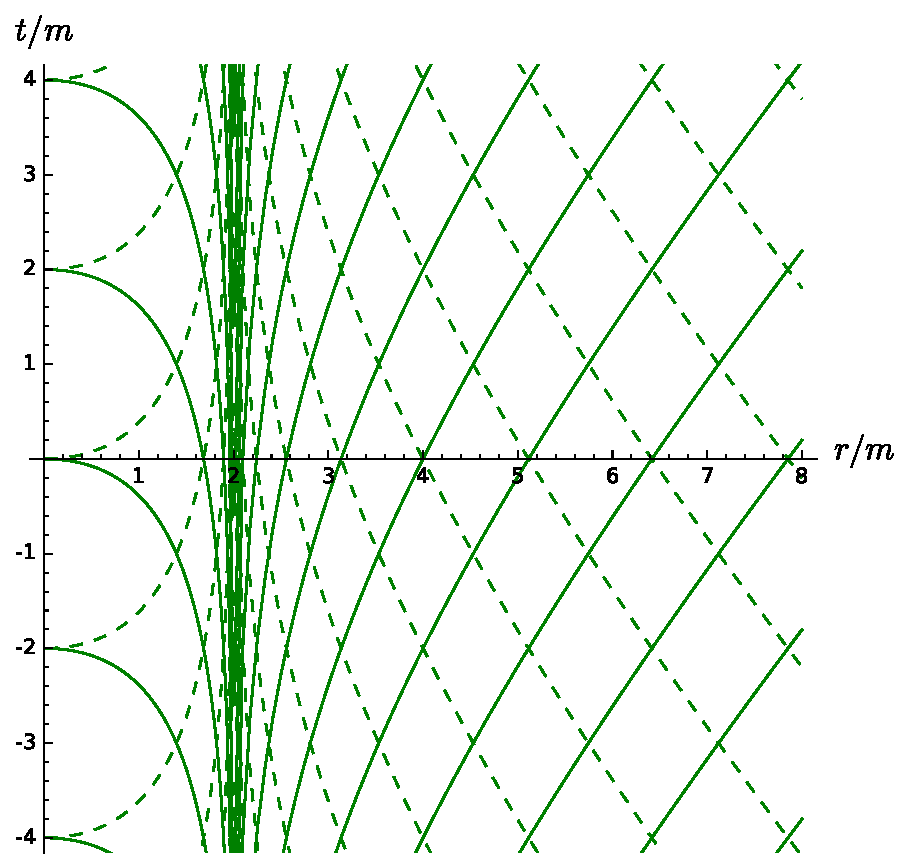
\includegraphics[width=0.6\textwidth]{sch_rad_null_geod.pdf}}
\caption[]{\label{f:sch:rad_null_geod} \footnotesize
Radial null geodesics of Schwarzschild spacetime, plotted in terms
of Schwarzschild-Droste coordinates $(t,r)$: the solid (resp. dashed) lines
correspond to outgoing (resp. ingoing) geodesics, as given by Eq.~(\ref{e:sch:outgoing_null_geod})
(resp. Eq.~(\ref{e:sch:ingoing_null_geod})). The interiors of some future light
cones are depicted in yellow.}
\end{figure}

\begin{itemize}
\item the \defin{outgoing radial null geodesics}\index{outgoing!null geodesic}, whose
equation is
\be \label{e:sch:outgoing_null_geod}
    t = r + 2 m \ln \left| \frac{r}{2m} - 1 \right| + u ,
\ee
where $u$ is a constant;
\item  the \defin{ingoing radial null geodesics}\index{ingoing!null geodesic}, whose
equation is
\be \label{e:sch:ingoing_null_geod}
    t = - r - 2 m \ln \left| \frac{r}{2m} - 1 \right| + v ,
\ee
where $v$ is a constant.
\end{itemize}

By introducing the \defin{tortoise coordinate}\index{tortoise coordinate}
\be \label{e:sch:def_tortoise}
    r_* := r + 2 m \ln \left| \frac{r}{2m} - 1 \right| ,
\ee
one may rewrite the above equations as
\bea
    &  & t = r_* + u \\
    &  & t = -r_* + v . \label{e:sch:v_advanced_tortoise}
\eea
The parameter $u$ appears then as a
\emph{retarded time}\index{retarded!time}\index{time!retarded --}:
$u = t - r_*$ and $v$ as an
\emph{advanced time}\index{advanced!time}\index{time!advanced --}: $v = t + r_*$.

Strictly speaking, we have found radial null \emph{curves} only, i.e. solutions of
Eq.~(\ref{e:sch:radial_null}). Since not all null curves
are geodesics\footnote{A famous counterexample is the helix in Minkowski
spacetime defined in terms of Minkowskian coordinates $(t,x,y,z)$ by $x = a\cos(t/a)$, $y = a\sin(t/a)$, $z=0$,
where $a$ is a positive constant. It is a null curve, but not a null geodesic.}, there remains to prove that the curves defined
by (\ref{e:sch:outgoing_null_geod}) and (\ref{e:sch:ingoing_null_geod})
obey the geodesic equation\index{geodesic!equation}:
\be \label{e:sch:geod_eqn}
    \frac{\D^2 x^\alpha}{\D \lambda^2} + \Gamma^\alpha_{\ \, \mu\nu}
        \derd{x^\mu}{\lambda} \derd{x^\nu}{\lambda} = 0 ,
\ee
where $\lambda$ is an affine parameter.
Let us check that (\ref{e:sch:geod_eqn}) is satisfied by choosing $\lambda=r$.
For the curves defined by (\ref{e:sch:outgoing_null_geod}), we have
\[
    x^\alpha(r) = \left( r + 2 m \ln \left| \frac{r}{2m} - 1 \right| + u,\ r,\  \th,\  \ph \right) .
\]
Hence
\[
    \derd{x^\alpha}{r} = \left( \frac{r}{r-2m}, 1, 0, 0 \right)
    \qquad\mbox{and}\qquad
    \frac{\D^2 x^\alpha}{\D r^2} = \left( - \frac{2m}{(r-2m)^2}, 0, 0, 0 \right) .
\]
Given the Christoffel symbols (\ref{e:sch:Christoffel_SD}), it is then a
simple exercice to show that Eq.~(\ref{e:sch:geod_eqn}) is satisfied.
The same property holds for the family (\ref{e:sch:ingoing_null_geod}). Hence
we conclude
\begin{greybox}
The radial null geodesics in the Schwarzschild-Droste domain are ruled by
Eqs.~(\ref{e:sch:outgoing_null_geod})-(\ref{e:sch:ingoing_null_geod}).
Moreover the areal radius $r$ is an affine parameter along them.
\end{greybox}

The two families of radial null geodesics are depicted in
Fig.~\ref{f:sch:rad_null_geod}.
The singularity of Schwarzschild-Droste coordinates at $r=2m$
is clearly apparent on this figure.


\begin{remark}
Despite their name, gedeosics of the outgoing family are actually
\emph{ingoing} in the region $r<2m$, in the sense that
$r$ is decreasing along them when moving towards the future. Indeed,
as noticed in Sec.~\ref{s:sch:SD_domain},
for $r<2m$, $r$ is the timelike coordinate of the system $(t,r,\th,\ph)$,
with $-\wpar_r$ oriented towards the future (cf. the ``tilted'' light cone
in Fig.~\ref{f:sch:rad_null_geod}).
\end{remark}

\subsection{Eddington-Finkelstein coordinates}

The parameter $v$ introduced in Eq.~(\ref{e:sch:ingoing_null_geod}) can be
seen as a label for the ingoing radial null geodesics: each of these curves is
entirely identified by the data $(v,\th,\ph)$, which remains fixed along it.
Let us promote $v$ to a spacetime coordinate, instead of $t$, i.e. let us
consider the coordinate system $(v,r,\th,\ph)$ with the relation to
Schwarzschild-Drostes coordinates $(t,r,\th,\ph)$ governed by Eq.~(\ref{e:sch:ingoing_null_geod}):
\be \label{e:sch:v_t_r}
     v = t + r + 2 m \ln \left| \frac{r}{2m} - 1 \right| .
\ee
It follows immediately that
\[
    \D v = \D t + \D r + \frac{\D r}{r/2m - 1} = \D t + \frac{\D r}{1 - 2m/r} ,
\]
i.e.
\[
    \D t = \D v -  \frac{\D r}{1 - 2m/r} .
\]
Taking the square gives
\[
    \D t^2 = \D v^2 - \frac{2}{1 - 2m/r} \, \D v \, \D r + \frac{1}{(1 - 2m/r)^2}\, \D r^2 .
\]
Substituting this expression for $\D t^2$ in Eq.~(\ref{e:sch:Schwarz_metric_SD})
yields the metric components with respect to the coordinates
$({\hat x}^\alpha) := (v,r,\th,\ph)$:
\be \label{e:sch:Schwarz_metric_NIEF}
    \encadre{
        {\hat g}_{\mu\nu}\, \D {\hat x}^\mu \, \D {\hat x}^\nu =
            -\left( 1 - \frac{2 m}{r} \right)\, \D v^2
            + 2 \, \D v \, \D r
        + r^2 \left( \D\th^2 + \sin^2\th\, \D\ph^2 \right) }.
\ee
The coordinates $({\hat x}^\alpha) = (v,r,\th,\ph)$ are called the
\defin{null ingoing Eddington-Finkelstein (NIEF) coordinates}\index{Eddington-Finkelstein!coordinates}\index{null!ingoing Eddington-Finkelstein coordinates}\index{NIEF}. The qualifier \emph{null} stems from the fact that
$r$ is a null coordinate in this system, i.e. the vector $\wpar_r$ of the coordinate
basis associated with $(v,r,\th,\ph)$ is a null
vector, as it follows from ${\hat g}_{rr}=0$ in Eq.~(\ref{e:sch:Schwarz_metric_NIEF}).

To deal with a ``standard'' time $+$ space coordinate system instead of a null one, let us set
\be  \label{e:sch:ti_v_r}
    \encadre{\ti := v - r} \iff \encadre{v = \ti + r}
\ee
and define the \defin{ingoing Eddington-Finkelstein (IEF) coordinates}\index{Eddington-Finkelstein!coordinates}\index{ingoing!Eddington-Finkelstein!coordinates}\index{IEF}
to be
\be
    (\tilde{x}^\alpha) := (\ti, r, \th,\ph) .
\ee

\begin{remark}
From (\ref{e:sch:ti_v_r}), $v$ appears as the ``time'' $\ti$ ``advanced'' by
$r$\index{advanced!time}\index{time!advanced --}, while
from (\ref{e:sch:v_advanced_tortoise}), $v$ is the ``time'' $t$ ``advanced''
by $r_*$.
\end{remark}

The relation between the ingoing Eddington-Finkelstein coordinates
$(\ti, r, \th,\ph)$
and the Schwarzschild-Droste ones $(t,r,\th,\ph)$ is obtained by combining
Eqs.~(\ref{e:sch:v_t_r}) and (\ref{e:sch:ti_v_r}):
\be \label{e:sch:ti_t_r}
     \encadre{\ti = t + 2 m \ln \left| \frac{r}{2m} - 1 \right| } .
\ee
The hypersurfaces $t=\mathrm{const}$ are plotted in Fig.~\ref{f:sch:SD_slices},
in terms of the IEF coordinates.

\begin{figure}
\centerline{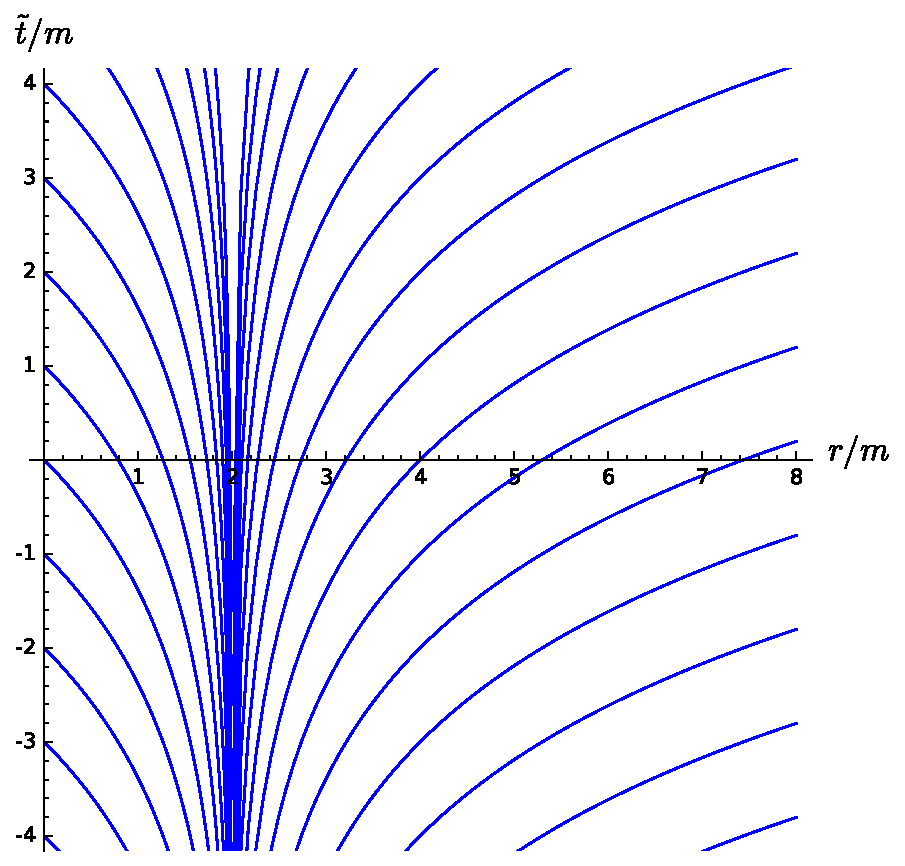
\includegraphics[width=0.6\textwidth]{sch_SD_slices.pdf}}
\caption[]{\label{f:sch:SD_slices} \footnotesize
Hypersurfaces of constant Schwarzschild-Droste coordinate $t$, drawn in term
of the ingoing Eddington-Finkelstein coordinates $(\ti,r)$. Since the dimensions
along $\th$ and $\ph$ are not represented, these 3-dimensional surfaces appear
as curves.}
\end{figure}

From (\ref{e:sch:ti_v_r}), we have $\D v = \D\ti + \D r$. Substituting
into (\ref{e:sch:Schwarz_metric_NIEF}) yields
\be \label{e:sch:Schwarz_metric_EF}
    \encadre{
        \tilde{g}_{\mu\nu}\, \D \tilde{x}^\mu \, \D \tilde {x}^\nu =
            -\left( 1 - \frac{2 m}{r} \right)\, \D \ti^2
            + \frac{4m}{r} \, \D \ti \, \D r
            + \left( 1 + \frac{2 m}{r} \right)\, \D r^2
        + r^2 \left( \D\th^2 + \sin^2\th\, \D\ph^2 \right) }.
\ee
We check that $\tilde{g}_{\ti\ti} < 0$ in $\M_{\rm I}$, hence $\ti$ is
a timelike coordinate there.
In $\M_{\rm II}$, $\tilde{g}_{\ti\ti} > 0$, so that $\ti$ becomes spacelike
there, as for the Schwarzschild-Droste coordinate $t$ (cf. Sec.~\ref{s:sch:SD_domain}).
However, we have $\tilde{g}_{rr} = 1+2m/r > 0$ everywhere, so that $r$ remains a spacelike coordinate (for the IEF system) in
$\M_{\rm II}$, contrary to what happens within the Schwarzschild-Droste coordinates
(cf. Sec.~\ref{s:sch:SD_domain}).

\begin{remark}
The above example shows that the property of being timelike, null or spacelike
is not intrinsic to a given coordinate (here $r$). It is instead a property
of the whole coordinate system under consideration. This is understandable
since $r$ spacelike means that the line along which $r$ varies while the
three other coordinates $(x^0,x^2,x^3)$ are kept constant is a spacelike curve.
For the Schwarzschild-Droste system $(x^0,x^2,x^3) = (t,\th,\ph)$,
while for the NIEF system
$(x^0,x^2,x^3) = (v,\th,\ph)$ and for
the IEF system $(x^0,x^2,x^3) = (\ti,\th,\ph)$.
Hence the three sets of $r$-lines differ.
Equivalently, the coordinate vectors $\wpar_r$
tangent to the three kinds of $r$-lines are different:
\[
    \left. \der{}{r} \right| _{t,\th,\ph} \not=
    \left. \der{}{r} \right| _{v,\th,\ph} \not=
    \left. \der{}{r} \right| _{\ti,\th,\ph} .
\]
\end{remark}
To avoid any ambiguity, we shall denote by $\wpar_{\tilde{r}}$ the
coordinate vector of the IEF frame and by
$\wpar_r$ the coordinate vector of the Schwarzschild-Droste frame:
\be
    \wpar_{\tilde{r}} := \left. \der{}{r} \right| _{\ti,\th,\ph}
    \qquad\mbox{and}\qquad
    \wpar_r := \left. \der{}{r} \right| _{t,\th,\ph} .
\ee
The relation between the two vectors is given by the chain rule:
\[
    \left. \der{}{r} \right| _{\ti,\th,\ph}  =
    \left. \der{}{t} \right| _{r,\th,\ph}
    \underbrace{ \left. \der{t}{r} \right| _{\ti,\th,\ph}}_{\left(1-\frac{r}{2m}\right)^{-1}}
  + \left. \der{}{r} \right| _{t,\th,\ph}
   \underbrace{\left. \der{r}{r} \right| _{\ti,\th,\ph}}_{1}
  + \left. \der{}{\th} \right| _{t,r,\ph}
  \underbrace{\left. \der{\th}{r} \right| _{\ti,\th,\ph}}_{0}
  + \left. \der{}{\ph} \right| _{t,r,\th}
  \underbrace{\left. \der{\ph}{r} \right| _{\ti,\th,\ph}}_{0} ,
\]
where (\ref{e:sch:ti_t_r}) has been used to evaluate
$\left. \dert{t}{r} \right| _{\ti,\th,\ph}$. Hence
\be
    \wpar_{\tilde{r}} = \wpar_r + \left(1-\frac{r}{2m}\right)^{-1} \, \wpar_t .
\ee

On the other hand, we deduce from (\ref{e:sch:ti_t_r}) that
\be
     \left. \der{}{\ti} \right| _{r,\th,\ph} = \left. \der{}{t} \right| _{r,\th,\ph} ,
\ee
which implies:
\be
    \wpar_{\ti} = \wpar_t .
\ee
In particular, the vector $\wpar_{\ti}$ of the IEF frame coincides with
the Killing vector $\w{\xi}$:
\be \label{e:sch:wparti_xi}
    \encadre{ \wpar_{\ti} = \w{\xi}} .
\ee
\begin{remark}
The result (\ref{e:sch:wparti_xi}) is not surprising since
the metric components (\ref{e:sch:Schwarz_metric_EF}) are independent from
$\ti$. This implies $\wpar_{\ti} = \alpha \w{\xi}$, where $\alpha$ is a constant.
Since $\ti \sim t$ when $r\rightarrow +\infty$, we conclude that $\alpha=1$.
\end{remark}

\begin{remark}
The IEF-coordinates line element (\ref{e:sch:Schwarz_metric_EF}) can be recast
in the following remarkable form:
\be \label{e:sch:Kerr_Schild}
    \tilde{g}_{\mu\nu}\, \D \tilde{x}^\mu \, \D \tilde {x}^\nu =
 \underbrace{- \D\ti^2 + \D r^2 + r^2  \left( \D\th^2 + \sin^2\th\, \D\ph^2 \right)}_{f_{\mu\nu} \, \D \tilde{x}^\mu \, \D \tilde {x}^\nu}
        + \underbrace{\frac{2m}{r} \left( \D\ti + \D r \right) ^2}_{k_\mu \D \tilde{x}^\mu \, k_\nu \D \tilde {x}^\nu} ,
\ee
where the $f_{\mu\nu}$'s are the components of the (flat) Minkowski metric expressed in
terms of the spherical coordinates $(\ti,r,\th,\ph)$ and the $k_\mu$'s are
the components of a 1-form dual to a null vector:
\[
    \uu{k} = \sqrt{\frac{2m}{r}} \, \dd (\ti + r) =
    \sqrt{\frac{2m}{r}} \, \dd v .
\]
The fact that $\w{k}$ is a null vector follows from
$g^{\mu\nu} k_\mu k_\nu = 0$, which is easily deduced from
$k_\mu = \sqrt{2m/r} (1, 1, 0, 0)$ and the expression (\ref{e:sch:inv_metric_EF})
of $g^{\mu\nu}$ below.
The line element (\ref{e:sch:Kerr_Schild}) is said to be of
\defin{Kerr-Schild form}\index{Kerr-Schild form}.
\end{remark}

\subsection{The Schwarzschild horizon} \label{s:sch:Schwarz_hor}

Contrary to the Schwarzschild-Droste components (\ref{e:sch:Schwarz_metric_SD}),
the metric components (\ref{e:sch:Schwarz_metric_EF}) are regular as
$r\rightarrow 2m$. In particular, their determinant is
\be
    \det\left( \tilde{g}_{\alpha\beta} \right) = - r^4\sin^2\th ,
\ee
which is never zero for $r\in(0,+\infty)$, except at the standard $\th=0$ and
$\th=\pi$ singularities of spherical coordinates.
The components of the inverse metric with respect to the ingoing
Eddington-Finkelstein coordinates are
\be \label{e:sch:inv_metric_EF}
    g^{\alpha\beta} = \left( \begin{array}{cccc}
    - \left( 1 + \frac{2m}{r} \right) &  \frac{2m}{r} & 0 & 0 \\[1ex]
    \frac{2m}{r} & 1 - \frac{2m}{r} & 0 & 0 \\[1ex]
    0 & 0 & \frac{1}{r^2} & 0 \\[1ex]
    0 & 0 & 0 & \frac{1}{r^2\sin^2\th}
    \end{array} \right) .
\ee
This proves that
(\ref{e:sch:Schwarz_metric_EF}) defines a regular non-degenerate metric
on the whole \defin{ingoing Eddington-Finkelstein domain}\index{ingoing!Eddington-Finkelstein!domain}
\be
    \M_{\rm IEF} := \R\times(0,+\infty)\times\SS^2,
\ee
with the coordinate $\ti$ spanning $\R$, the coordinate $r$ spanning
$(0,+\infty)$ and the coordinates $(\th,\ph)$ forming a standard spherical
chart of $\SS^2$.
The IEF domain is an extension of the Schwarzschild-Droste domain
introduced in Sec.~\ref{s:sch:SD_domain}:
\be
    \M_{\rm IEF} = \M_{\rm SD} \cup \Hor = \M_{\rm I} \cup \M_{\rm II} \cup \Hor ,
\ee
where $\Hor$ is the subset of $\M_{\rm IEF}$ defined by $r=2m$. Note that
$\Hor$ has the topology
\be
    \Hor \simeq \R\times\SS^2
\ee
and that $(\ti,\th,\ph)$ is a coordinate system on $\Hor$.
Actually $\Hor$ is nothing but what has been called the
\defin{Schwarzschild horizon}\index{Schwarzschild!horizon} in the examples
of Chaps.~\ref{s:def} and \ref{s:neh}. Indeed, the metric
(\ref{e:sch:Schwarz_metric_EF}) is nothing but
the metric (\ref{e:def:Schw_metric}) introduced in Example~\ref{x:def:Schw_hor}
of Chap.~\ref{s:def} (p.~\pageref{x:def:Schw_hor}), up to the change of notation $\ti \leftrightarrow t$ (compare (\ref{e:def:Schw_metric_inv}) and
(\ref{e:sch:inv_metric_EF}) as well).
We have thus the fundamental result,
the proof of which is given in Example~\ref{x:neh:Schwarz_KH} of Chap.~\ref{s:neh}
(p.~\pageref{x:neh:Schwarz_KH}):
\begin{greybox}
$\Hor$ is a Killing horizon, the null normal of which is $\w{\xi}$.
\end{greybox}
In particular, $\Hor$ is a null hypersurface, whose null geodesic generators
admit $\w{\xi} = \wpar_{\ti}$ as tangent vector. It is a non-expanding horizon,
whose area, as defined in Sec.~\ref{s:neh:invar_area}, is (cf. Example~\ref{x:neh:Schwarz_hor_area} of Chap.~\ref{s:neh}, p.~\pageref{x:neh:Schwarz_hor_area})
\be
    A=16\pi m^2 .
\ee
$\Hor$ is depicted in Fig.~\ref{f:def:Schwarz_horizon}.
We shall see in Sec.~?? that $\Hor$ is actually a black hole event horizon in
Schwarzschild spacetime.

\subsection{Coordinate singularity vs. curvature singularity}
\label{s:sch:singularities}

The above considerations show that the divergence of the metric
component $g_{rr}$ in (\ref{e:sch:Schwarz_metric_SD}) when $r\rightarrow 2m$
reflects a pathology of Schwarzschild-Droste coordinates and not a singularity
in the metric tensor $\w{g}$ by itself: $(\M_{\rm IEF}, \w{g})$ is perfectly
regular spacetime, including at $r=2m$.
The bad behaviour of of Schwarzschild-Droste coordinates is obvious in Fig.~\ref{f:sch:SD_slices}: the hypersurfaces
$t=\mathrm{const}$ fail to provide a regular slicing of spacetime.
This pathology is called a
\defin{coordinate singularity}\index{coordinate!singularity}\index{singularity!coordinate --}, since it is intrinsic a given coordinate system
(here the Schwarzschild-Droste one).

Another pathology appears in the metric components in both the Schwarzschild-Droste coordinates and the ingoing Eddington-Finkelstein ones: $g_{tt}$ and $\tilde{g}_{\ti\ti}$ diverge when $r\rightarrow 0$. This type of singularity
cannot be removed by a coordinate transformation. Indeed the
\defin{Kretschmann scalar}\index{Kretschmann scalar}, defined as the
following ``square'' of the Riemann curvature tensor
\be \label{e:sch:def_Kretschmann}
    K := R_{\mu\nu\rho\sigma} R^{\mu\nu\rho\sigma} ,
\ee
is (cf. Appendix~?? for the computation})
\be
    K = \frac{48 m^2}{r^6} .
\ee
Hence $K\rightarrow +\infty$ when $r\rightarrow 0$. Since $K$ is a scalar
field, its value is independent of any coordinate system used to express it.
Hence the divergence of $K$ reflects a pathology of the Riemann tensor
per se: it is called a
\defin{curvature singularity}\index{curvature!singularity}\index{singularity!curvature --}.


\begin{hist}
Eddington-Finkelstein coordinates have been introduced by
Arthur Eddington in 1924 \cite{Eddin1924}. More precisely, Eddington
introduced the \emph{outgoing} version of these coordinates,
while we have focussed above on the \emph{ingoing} version. Indeed
Eddington's Eq.~(2) is $\ti = t - 2m \ln(r-m)$, which mainly differs from
our Eq.~(\ref{e:sch:ti_t_r}) by the minus sign in front of the logarithm\footnote{The other differences with (\ref{e:sch:ti_t_r}) are a constant additive term
and a misprint in Eddington's formula: the term $\ln(r-m)$ should be replaced
by $\ln(r-2m)$.},
which means that Eddington's time coordinate is actually $\ti = u + r$, instead of
$\ti = v - r$ (our Eq.~(\ref{e:sch:ti_v_r})). Eddington used his transformation
to get the Kerr-Schild form (\ref{e:sch:Kerr_Schild}) of Schwarzschild metric,
with $(\D \ti + \D r)^2$ replaced by $(\D \ti - \D r)^2$ due to the change
ingoing $\leftrightarrow$ outgoing. For a modern reader, it is quite surprising
that Eddington did not point out that the metric components w.r.t. $(\ti,r,\th,\ph)$
are regular at $r=2m$. Actually the main purpose of Eddington's article
\cite{Eddin1924} was elsewhere, in the comparison of general relativity to an alternative theory proposed in 1922 by the mathematician Alfred N. Whitehead
(see e.g. \cite{GibboW08}).
Only in 1958 did David Finkelstein reintroduce the Eddington transformation
to demonstrate that the Schwarzschild metric is analytic over the whole domain
$r\in(0,+\infty)$ \cite{Finke58}. Meanwhile the regularity of Schwarzschild metric
at $r=2m$ had been proved by Georges Lemaître in 1932 \cite{Lemai32}, by means of
another coordinate system (see \cite{Eisen93} for a detailed discussion).
\end{hist}

\begin{remark}
In the literature, the terminology \emph{Eddington-Finkelstein coordinates}
is often used for the coordinates $(v,r,\th,\ph)$ (or $(u,r,\th,\ph)$),
i.e. for what we have called the \emph{null Eddington-Finkelstein coordinates},
and the regularity of the metric tensor at $r=2m$ is demonstrated by
considering the components (\ref{e:sch:Schwarz_metric_NIEF}).
However, neither
Eddington \cite{Eddin1924} nor Finkelstein \cite{Finke58}
considered this null version: they used coordinates $(\ti,r,\th,\ph)$, where
$\ti$ is timelike and they exhibited (the outgoing version of) the
metric components (\ref{e:sch:Schwarz_metric_EF}).
Hence our terminology is more faithfull to history. Moreover, focussing on
$(v,r,\th,\ph)$ may give the false impression to a novice reader that it is
necessary to introduce some null coordinate to establish the regularity
of the metric tensor at $r=2m$, while the timelike coordinate $\ti$
does the job very well.
\end{remark}

\begin{figure}
\centerline{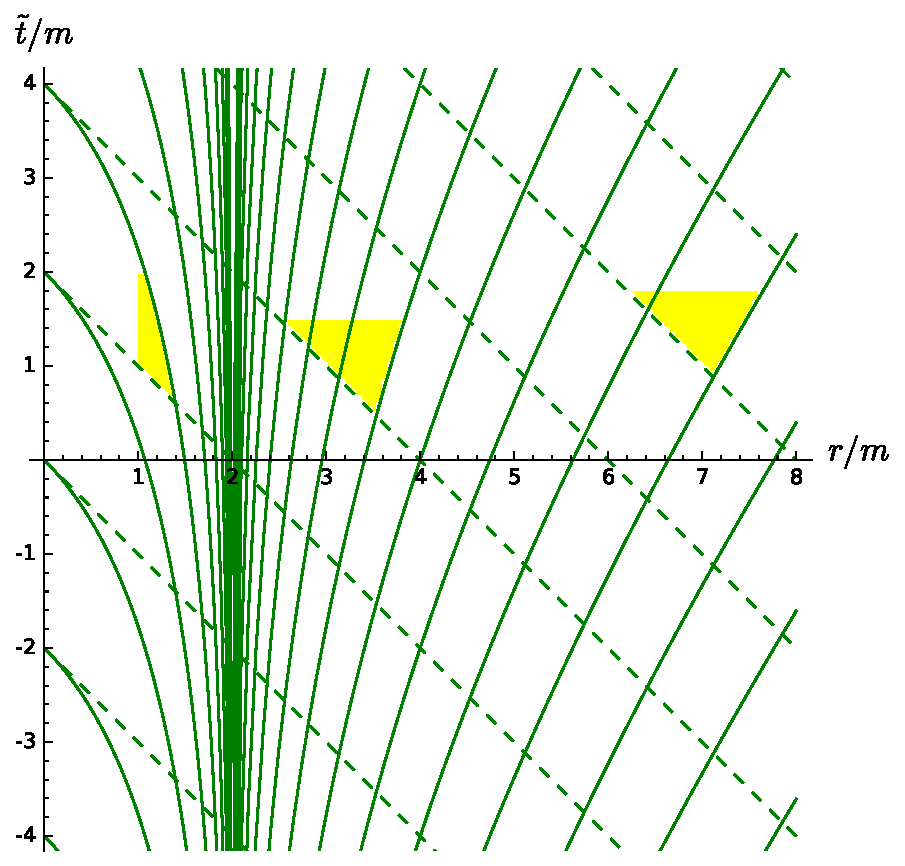
\includegraphics[width=0.6\textwidth]{sch_rad_null_geod_EF.pdf}}
\caption[]{\label{f:sch:rad_null_geod_EF} \footnotesize
Radial null geodesics of Schwarzschild spacetime, plotted in terms
of ingoing Eddington-Finkelstein coordinates $(\ti,r)$: the solid (resp. dashed) lines
correspond to outgoing (resp. ingoing) geodesics, as given by Eq.~(\ref{e:sch:outgoing_null_geod_EF})
(resp. Eq.~(\ref{e:sch:ingoing_null_geod_EF})). The interiors of some future light
cones are depicted in yellow.}
\end{figure}

\subsection{Radial null geodesics in terms of the Eddington-Finkelstein coordinates}

By construction, the equation of the ingoing radial null geodesics
in terms of the IEF coordinates is very simple:
\be \label{e:sch:ingoing_null_geod_EF}
    \ti = - r + v ,
\ee
where the constant $v\in \R$ labels the geodesic.
The equation of the outgoing radial null geodesics is obtained
by combining (\ref{e:sch:outgoing_null_geod}) and (\ref{e:sch:ti_t_r}):
\be \label{e:sch:outgoing_null_geod_EF}
    \ti = r + 4 m \ln \left| \frac{r}{2m} - 1 \right| + u ,
\ee
where the constant $u\in \R$ labels the geodesic.
The radial null geodesics are depicted in Fig.~\ref{f:sch:rad_null_geod_EF}
in terms of the IEF coordinates. We note that, contrary to Fig.~\ref{f:sch:rad_null_geod},
which was based on Schwarzschild-Drostes coordinates, in the region $r<2m$,
the future light cones point upwards. This reflects the fact that, in the IEF system,
$\ti$ is a timelike coordinate and $r$ a spacelike one.

%%%%%%%%%%%%%%%%%%%%%%%%%%%%%%%%%%%%%%%%%%%%%%%%%%%%%%%%%%%%%%%%%%%%%%%%%%%%%%%

\section{Maximal extension}

\subsection{Kruskal-Szekeres coordinates} \label{s:sch:KS_coord}

On the open set $\M_{\rm I}$, let us consider the ``double-null''
coordinate system $\hat{\hat{x}}^\alpha = (u,v,\th,\ph)$. It is related to
Schwarzschild-Droste coordinates $(t,r,\th,\ph)$ by
Eqs.~(\ref{e:sch:outgoing_null_geod})-(\ref{e:sch:ingoing_null_geod}):
\be \label{e:sch:u_v_r_t}
    \left\{\begin{array}{l}
    u = t - r - 2 m \ln \left| \frac{r}{2m} - 1 \right| \\[1ex]
    v = t + r + 2 m \ln \left| \frac{r}{2m} - 1 \right|
    \end{array}\right.
    \iff
        \left\{\begin{array}{l}
    t = \frac{1}{2} (u+v)\\[1ex]
    r + 2 m \ln \left| \frac{r}{2m} - 1 \right| = \frac{1}{2} (v-u).
    \end{array}\right.
\ee
Despite one cannot express explicitely $r$ in terms of $(u,v)$,
the function $r\mapsto r + 2 m \ln \left| \frac{r}{2m} - 1 \right|$ is
invertible on $(2m,+\infty)$ (cf. Fig.~\ref{f:sch:tortoise}), so that (\ref{e:sch:u_v_r_t}) does define a coordinate system on $\M_{\rm I}$.
The range of $(u,v)$ is $\R^2$.

The above relations imply
\[
 \D u = \D t - \frac{\D r}{1 - \frac{2m}{r}}  \qquad\mbox{and}\qquad
\D v = \D t + \frac{\D r}{1 - \frac{2m}{r}} .
\]
Hence
\[
    \D u \, \D v = \D t^2 - \frac{\D r^2}{\left(1 - \frac{2m}{r} \right) ^2} .
\]
The line element (\ref{e:sch:Schwarz_metric_SD}) becomes then
\be \label{e:sch:Schwarz_metric_uv}
    \encadre{
        \hat{\hat{g}}_{\mu\nu}\, \D \hat{\hat{x}}^\mu \,
        \D \hat{\hat{x}}^\nu =
            -\left( 1 - \frac{2 m}{r} \right)\, \D u \, \D v
       +  r^2 \left( \D\th^2 + \sin^2\th\, \D\ph^2 \right) }.
\ee
In this formula, $r$ is to be considered as a function of $(u,v)$, given
by (\ref{e:sch:u_v_r_t}).

\begin{figure}
\centerline{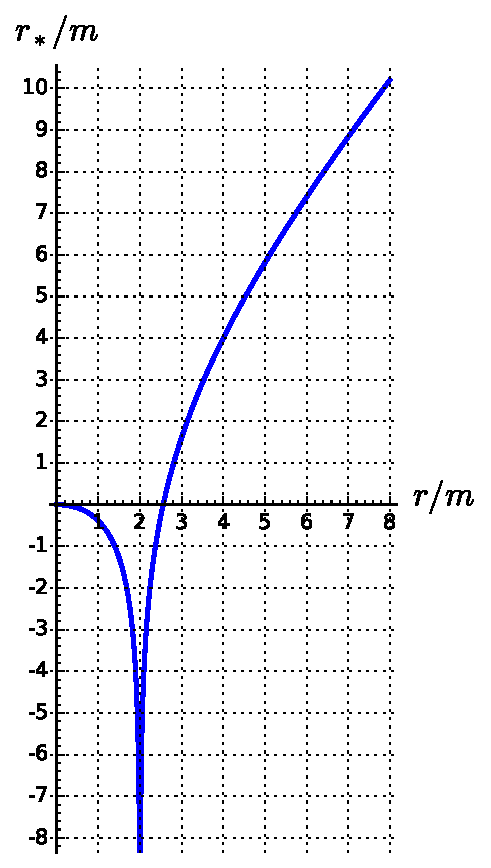
\includegraphics[height=0.4\textheight]{sch_tortoise.pdf}}
\caption[]{\label{f:sch:tortoise} \footnotesize
Function $r_*(r) = r + 2 m \ln \left| \frac{r}{2m} - 1 \right|$
(the tortoise coordinate, cf. Eq.~(\ref{e:sch:def_tortoise})).
It relates $r$ to $(u,v)$ via $r_*(r) = (u-v)/2$ [Eq.~(\ref{e:sch:u_v_r_t})].}
\end{figure}

The metric components (\ref{e:sch:Schwarz_metric_uv}) are regular on $\M_{\rm I}$.
Having a look at Fig.~\ref{f:sch:tortoise}, we realize that we cannot extend
this coordinate system to include the Schwarzschild horizon $\Hor$, since
$r\rightarrow 2m$ is equivalent to $v-u\rightarrow -\infty$: if $u$ (resp. $v$)
were taking a finite value on $\Hor$, we would have $v\rightarrow -\infty$
(resp. $u\rightarrow +\infty$). This impossibility of extending to $\Hor$
is also reflected by the fact that
\[
    \det \left( \hat{\hat{g}}_{\alpha\beta} \right) =
        - \frac{1}{4} \left( 1 - \frac{2 m}{r} \right) ^2 r^4 \sin^2\th
\]
vanishes for $r\rightarrow 2m$, which would make $\w{g}$ a degenerate bilinear
form at $r=2m$, which is not of course.

Instead of $(u,v)$, let us use on $\M_{\rm I}$
the coordinates $(U,V)$ defined by
\be \label{e:sch:def_U_V}
    \left\{\begin{array}{l}
    U := - \mathrm{e}^{-u/4m} \\
    V := \mathrm{e}^{v/4m} .
    \end{array}\right.
\ee
Since the range of $(u,v)$ is $\R^2$, the range of $U$ is $(-\infty,0)$
and that of $V$ is $(0,+\infty)$.
We have
\[
    \D U = \frac{1}{4m} \,  \mathrm{e}^{-u/4m}  \, \D u\qquad\mbox{and}\qquad
    \D V = \frac{1}{4m} \,  \mathrm{e}^{v/4m} \, \D v ,
\]
hence
\[
    \D u \, \D v = 16 m^2 \mathrm{e}^{(u-v)/4m} \, \D U \, \D V .
\]
Now, on $\M_{\rm I}$, $r>2m$ and (\ref{e:sch:u_v_r_t}) yields
\be \label{e:sch:r_u_v_exp}
    r + 2 m \ln \left( \frac{r}{2m} - 1 \right) = \frac{1}{2} (v-u)
    \quad
    \Longrightarrow
    \quad
     \mathrm{e}^{r/2m} \left( \frac{r}{2m} - 1 \right)  =
    \mathrm{e}^{(v-u)/4m}  ,
\ee
so that
\[
     \D u \, \D v = 16 m^2 \, \mathrm{e}^{-r/2m}
        \left( \frac{r}{2m} - 1 \right) ^{-1} \D U \, \D V
        = \frac{32 m^3}{r} \, \mathrm{e}^{-r/2m}
        \left( 1 - \frac{2m}{r} \right) ^{-1} \D U \, \D V .
\]
Substituting this expression in (\ref{e:sch:Schwarz_metric_uv}) yields
the expression of the metric components with respect to
coordinates ${\hat X}^\alpha := (U,V,\th,\ph)$:
\be \label{e:sch:metric_UV}
    \encadre{
    g_{\mu\nu} \, \D {\hat X}^\mu \, \D {\hat X}^\nu =
    - \frac{32 m^3}{r} \, \mathrm{e}^{-r/2m} \,  \D U \, \D V
     +  r^2 \left( \D\th^2 + \sin^2\th\, \D\ph^2 \right) }.
\ee
In this formula, $r$ has to be considered as a function of $(U,V)$, whose
implicit expression is found by combining
(\ref{e:sch:def_U_V}) and (\ref{e:sch:r_u_v_exp}):
\be \label{e:sch:r_UV}
    \encadre{ \mathrm{e}^{r/2m} \left( \frac{r}{2m} - 1 \right) = - U V } .
\ee
\begin{remark}
This relation takes a very simple form in terms of the tortoise coordinate
(cf. Eq.~(\ref{e:sch:def_tortoise})):
\[
    \mathrm{e}^{r_*/2m} = - U V  .
\]
\end{remark}

We notice that the factor $(1-2m/r)$ has disappeared in the line
element (\ref{e:sch:metric_UV}), which becomes perfectly regular as
$r\rightarrow 2m$.

We read on (\ref{e:sch:metric_UV}) that $g_{UU} = 0$ and $g_{VV} = 0$.
Hence $(U,V)$ is a double-null coordinate system, as much as $(u,v)$.
To cope with a timelike-spacelike coordinate system instead, let
us introduce on $\M_{\rm I}$ the pair $(T,X)$ such that $U$ is $T$
retarded by $X$ and $V$ is $T$ advanced by $X$:
\be \label{e:sch:def_T_X}
    \left\{\begin{array}{l}
    U = T - X\\
    V = T + X
    \end{array}\right.
    \qquad \iff\qquad
    \left\{\begin{array}{l}
    T = \frac{1}{2} (U+V) \\[1ex]
    X = \frac{1}{2} (V-U)
    \end{array}\right.
\ee
Since the range of $U$ on $\M_{\rm I}$ is $(-\infty,0)$ and that of $V$ is
$(0,+\infty)$, the range of $(T,X)$ is ruled by $T<X$, $T>-X$ and $X>0$.
In other words, the coordinates $(T,X)$ span the following quarter of
$\mathbb{R}^2$ (cf. Fig.~\ref{f:sch:SD_I_KS}):
\be \label{e:sch:X_T_range_I}
    \M_{\rm I}: \quad X > 0 \quad\mbox{and}\quad -X < T < X .
\ee
The coordinates $X^\alpha := (T,X,\th,\ph)$ are called
the \defin{Kruskal-Szekeres coordinates}\index{Kruskal-Szekeres!coordinates}.

\begin{figure}
\centerline{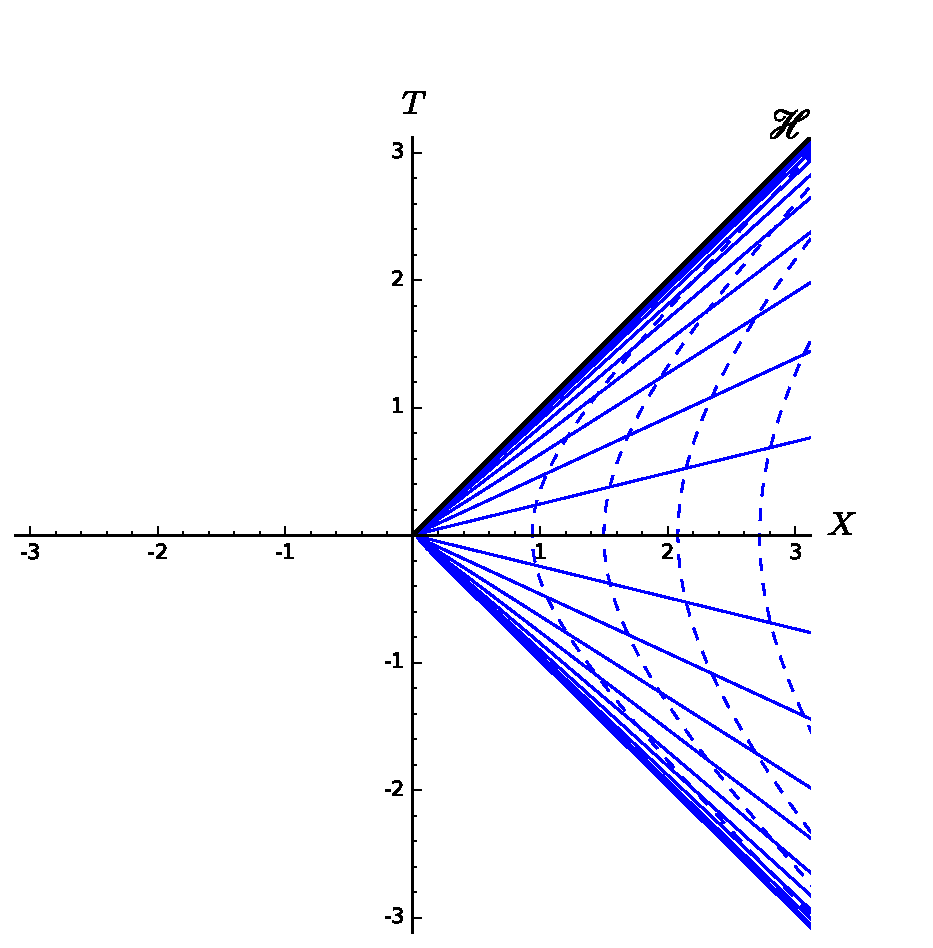
\includegraphics[width=0.6\textwidth]{sch_SD_I_KS.pdf}}
\caption[]{\label{f:sch:SD_I_KS} \footnotesize
Submanifold $\M_{\rm I}$ in the Kruskal-Szekeres coordinates $(T,X)$:
$\M_{\rm I}$ is covered by the Schwarzschild-Droste grid (in blue): the solid
lines have $t=\mathrm{const}$ (spaced apart by $\delta t = m$), while the
dashed curves have $r=\mathrm{const}$ (spaced apart by $\delta r = m/2$).}
\end{figure}


We have $\D U \, \D V = (\D T - \D X) (\D T + \D X)  = \D T^2 - \D X^2$,
so that the metric components with respect to the Kruskal-Szekeres coordinates
are easily deduced from the line element (\ref{e:sch:metric_UV}):
\be \label{e:sch:metric_KS}
    \encadre{
    g_{\mu\nu} \, \D X^\mu \, \D X^\nu =
    \frac{32 m^3}{r} \, \mathrm{e}^{-r/2m}
    \left( - \D T^2 + \D X^2 \right)
     +  r^2 \left( \D\th^2 + \sin^2\th\, \D\ph^2 \right) }.
\ee
Here $r$ is to be considered as the function of $(T,X)$ that is defined
implicitely by
\be \label{e:sch:X2mT2}
   \encadre{ \mathrm{e}^{r/2m} \left( \frac{r}{2m} - 1 \right) = X^2 - T^2 } .
\ee
This relation is a direct consequence of (\ref{e:sch:r_UV}) and (\ref{e:sch:def_T_X}).
We may rewrite it as $F(r/2m) = X^2 - T^2$, with $F$ being the function
defined by
\be \label{e:sch:def_F}
    \begin{array}{cccc}
    F: & (0,+\infty) & \longrightarrow & (-1,+\infty) \\
        & x & \longmapsto & \mathrm{e}^{x} ( x - 1 ) .
    \end{array}
\ee
The graph of $F$  is shown in Fig.~\ref{f:sch:X2mT2}. We see clearly that it is a bijective map.
In particular, $F$ induces a bijection between $(1,+\infty)$ (the range of $r/2m$ on $\M_{\rm I}$)
and $(0,+\infty)$ (the range of $X^2-T^2$ on $\M_{\rm I}$, according to (\ref{e:sch:X_T_range_I})).
Hence, in the line element (\ref{e:sch:metric_KS}), we may write
$r = 2m F^{-1}(X^2-T^2)$. Noticing that
$2m/r \, \mathrm{e}^{-r/2m} = (X^2-T^2 + \mathrm{e}^{r/2m})^{-1}$
[cf. Eq.~(\ref{e:sch:X2mT2})], we may eliminate $r$ from the expression
of the metric components in Kruskal-Szekeres coordinates:
\be \label{e:sch:metric_KS_TX}
   \encadre{
    \begin{array}{lcll}
    g_{\mu\nu} \, \D X^\mu \, \D X^\nu & = & 4m^2 \bigg\{ & \displaystyle
    \frac{4}{X^2-T^2 + \mathrm{e}^{F^{-1}(X^2-T^2)} }
    \left( - \D T^2 + \D X^2 \right) \\[2ex]
    & & & \displaystyle + \,   (F^{-1}(X^2-T^2))^2 \left( \D\th^2 + \sin^2\th\, \D\ph^2 \right)
    \bigg\}.
    \end{array} }
\ee




\begin{figure}
\centerline{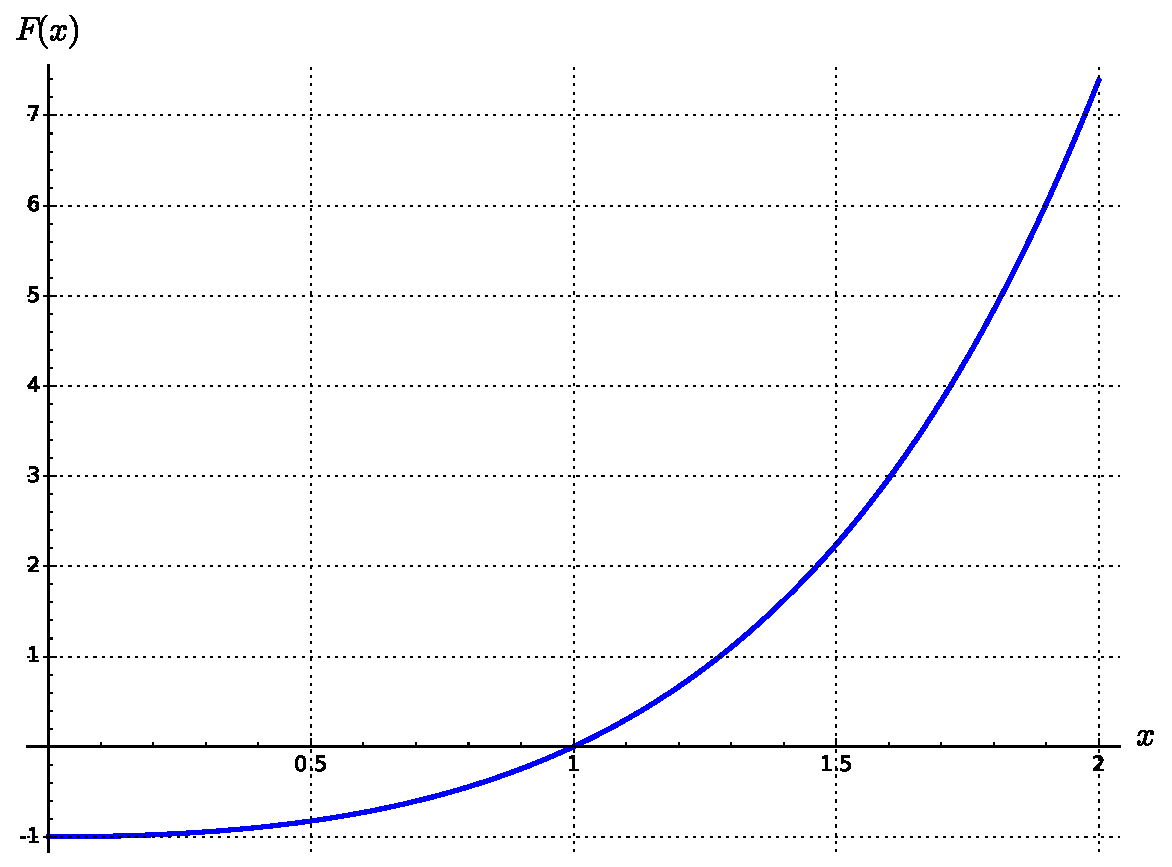
\includegraphics[height=0.37\textheight]{sch_X2mT2.pdf}}
\caption[]{\label{f:sch:X2mT2} \footnotesize
Function $F(x) = \mathrm{e}^{x} (x-1)$, giving
$X^2-T^2 = F(r/2m)$, cf. Eq.~(\ref{e:sch:X2mT2}).}
\end{figure}


The relation between the Kruskal-Szekeres coordinates and the
Schwarzschild-Droste ones is obtained by combining (\ref{e:sch:def_T_X}),
(\ref{e:sch:def_U_V}) and (\ref{e:sch:u_v_r_t}):
\bea
    T &=& \frac{1}{2}(U+V) = \frac{1}{2} \left( \mathrm{e}^{v/4m}
        - \mathrm{e}^{-u/4m)} \right) =
        \frac{1}{2} \left( \mathrm{e}^{(t+r_*)/4m}
        - \mathrm{e}^{(r_*-t)/4m} \right) \nonumber \\
     & = & \mathrm{e}^{r_*/4m} \sinh\left( \frac{t}{4m} \right) ,\nonumber
\eea
where $r_*$ is related to $r$ by (\ref{e:sch:def_tortoise}).
Similarly
\[
     X = \mathrm{e}^{r_*/4m} \cosh\left( \frac{t}{4m} \right) .
\]
In particular, we have
\[
    \frac{T}{X} = \tanh\left( \frac{t}{4m} \right) .
\]
From Eq.~(\ref{e:sch:def_tortoise}), we have
\[
    \mathrm{e}^{r_*/4m} = \mathrm{e}^{r/4m} \sqrt{ \frac{r}{2m} - 1 } .
\]
We may summarize the above relations as follows:
\be \label{e:sch:KS_SD_I}
    \M_{\rm I}: \quad \encadre{ \left\{\begin{array}{l}
    T = \mathrm{e}^{r/4m} \sqrt{ \frac{r}{2m} - 1 } \sinh\left( \frac{t}{4m} \right)
\\[2ex]
    X = \mathrm{e}^{r/4m} \sqrt{ \frac{r}{2m} - 1 } \cosh\left( \frac{t}{4m} \right)
        \end{array}\right. }
    \iff
    \encadre{ \left\{\begin{array}{l}
    t = 2 m \,  \ln \left( \frac{X+T}{X-T} \right) \\[2ex]
    r = 2 m F^{-1}(X^2 - T^2) .
        \end{array}\right. }
\ee
Note that we have used the identity $\mathrm{artanh}\, x = 1/2 \ln\left[(1+x)/(1-x)\right]$.
The curves of constant $t$ and constant $r$ in the $(T,X)$ plane
are drawn in Fig.~\ref{f:sch:SD_I_KS}.
\begin{remark}
Given the properties of the $\cosh$ and $\sinh$ functions, it is clear on these
expressions that the constraints (\ref{e:sch:X_T_range_I}) are satisfied.
\end{remark}
\begin{remark}
In line element (\ref{e:sch:metric_KS_TX})
the metric components $g_{TT}$ and $g_{XX}$ depend on both $X$ and $T$; this
shows that neither $\wpar_T$ nor $\wpar_X$ coincide with a Killing vector.
In other words, the coordinates $(T,X)$ are not adapted to the spacetime
symmetries, contrary to the Schwarzschild-Droste coordinates or to the
Eddington-Finkelstein ones.
\end{remark}

\subsection{Extension to the IEF domain}

We notice that the metric components (\ref{e:sch:metric_KS}) are perfectly
regular at $r=2m$. Therefore the Kruskal-Szekeres coordinates can be extended
to cover the Schwarzschild horizon $\Hor$. Actually they can be extended to
all values of $r\in (0,2m]$, i.e. to the whole domain of the ingoing
Eddington-Finkelstein coordinates: the manifold $\M_{\rm IEF}$ introduced
in Sec.~\ref{s:sch:Schwarz_hor}:
$\M_{\rm IEF} = \M_{\rm I} \cup \Hor \cup \M_{\rm II}$. Let us show
this in detail. Back on $\M_{\rm I}$, we can express the IEF coordinate
$\ti$ in terms of $(T,X)$ by combining $\ti = v - r$ [Eq.~(\ref{e:sch:ti_v_r})],
$v = 4m\ln V$ [Eq.~(\ref{e:sch:def_U_V})] and $V = T+X$ [Eq.~(\ref{e:sch:def_T_X})]:
\be
    \ti = 4 m \ln (T+X) - r.
\ee
The above relation is a valid expression as long as $T+X>0$.
Besides, we already noticed
that the function $F$ defined by (\ref{e:sch:def_F}) is a bijection from the range of $r/2m$
on $\M_{\rm IEF}$, i.e. $(0,+\infty)$, to $(-1,+\infty)$, with the
$(0,+\infty)$ part of the latter interval representing the range of $X^2-T^2$
on $\M_{\rm I}$. We may use these properties to extend the Kruskal-Szekeres coordinates to all $\M_{\rm IEF}$ by requiring
\begin{subequations}
\label{e:sch:ti_r_X_T}
\begin{align}
 & \ti = 4 m \ln (T+X) - r\\
 & \underbrace{\mathrm{e}^{r/2m} \left( \frac{r}{2m} - 1 \right)}_{F(r/2m)} = X^2-T^2 .
 \end{align}
\end{subequations}
The range of the coordinates $(T,X)$ on $\M_{\rm IEF}$ is then ruled by
\[
    \M_{\rm IEF}:\quad T+X > 0 \quad\mbox{and}\quad X^2 - T^2 > -1 ,
\]
which can be rewritten as
\be \label{e:sch:range_X_T_IEF}
    \M_{\rm IEF}: \quad -X < T < \sqrt{X^2+1}.
\ee
We deduce from (\ref{e:sch:ti_r_X_T}) that
\be \label{e:sch:KS_IEF_prov}
    \left\{\begin{array}{lcl}
    X+T & = & \mathrm{e}^{(\ti+r)/4m} \\
    X-T & = & \mathrm{e}^{(r -\ti)/4m} \left( \frac{r}{2m} - 1 \right) .
    \end{array}\right.
\ee
Hence the relation between the ingoing Eddington-Finkelstein coordinates and
the Kruskal-Szekeres ones on $\M_{\rm IEF}$:
\be \label{e:sch:KS_IEF}
    \encadre{ \left\{\begin{array}{l}
    T = \mathrm{e}^{r/4m} \left[ \cosh\left(\frac{\ti}{4m}\right)
        - \frac{r}{4m} \mathrm{e}^{-\ti/4m} \right] \\[2ex]
    X =  \mathrm{e}^{r/4m} \left[ \sinh\left(\frac{\ti}{4m}\right)
        + \frac{r}{4m} \mathrm{e}^{-\ti/4m}  \right]
    \end{array}\right. }
    \iff
    \encadre{\left\{\begin{array}{l}
     \ti =  2 m \left[ 2 \ln (T+X) - F^{-1}(X^2 - T^2) \right] \\[1ex]
    r = 2 m F^{-1}(X^2 - T^2)
    \end{array}\right. }
\ee
The various subsets of $\M_{\rm IEF}$ correspond then to the following
coordinate ranges (cf. Fig.~\ref{f:sch:IEF_KS}):
\begin{subequations}
\begin{align}
 & \M_{\rm I}: \quad X > 0 \quad\mbox{and}\quad -X < T < X \\
 & \Hor: \quad X > 0 \quad\mbox{and}\quad  T = X \\
 & \M_{\rm II}: \quad |X| < T < \sqrt{X^2+1} .
\end{align}
\end{subequations}

\begin{figure}
\centerline{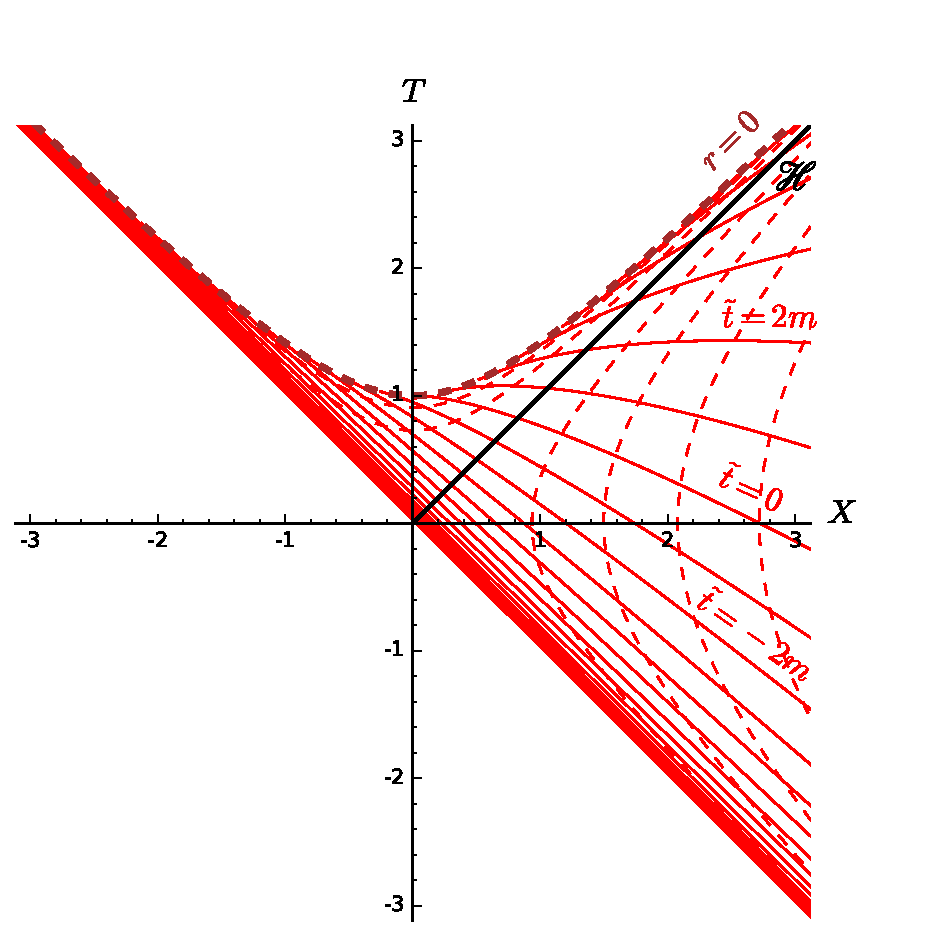
\includegraphics[width=0.6\textwidth]{sch_IEF_KS.pdf}}
\caption[]{\label{f:sch:IEF_KS} \footnotesize
Domain of ingoing Eddington-Finkelstein coordinates, $\M_{\rm IEF} = \M_{\rm I}\cup \Hor\cup \M_{\rm II}$, depicted in terms of the Kruskal-Szekeres coordinates $(T,X)$: the solid red
curves have $\ti=\mathrm{const}$ (spaced apart by $\delta\ti = m$), while the
dashed red curves have $r=\mathrm{const}$ (spaced apart by $\delta r = m/2$).}
\end{figure}


Since the relation between IEF coordinates and Kruskal-Szekeres ones is the
same in $\M_{\rm II}$ as in $\M_{\rm I}$ (being given by (\ref{e:sch:KS_IEF})
in both cases), we conclude that the expression (\ref{e:sch:metric_KS})
of the metric components with respect to
Kruskal-Szekeres coordinates is valid in all $\M_{\rm IEF}$.

Let us determine the relation between the Kruskal-Szekeres coordinates and
the Schwarz\-schild-Droste ones in $\M_{\rm II}$. Since $r<2m$ in $\M_{\rm II}$,
Eq.~(\ref{e:sch:ti_t_r}) gives
\[
    \M_{\rm II}: \quad  \mathrm{e}^{\ti/4m} = \mathrm{e}^{t/4m}  \sqrt{1 -  \frac{r}{2m} } ,
\]
so that (\ref{e:sch:KS_IEF_prov}) can be rewritten as
\[
     \M_{\rm II}: \quad
\left\{\begin{array}{lcl}
    X+T & = & \displaystyle \mathrm{e}^{(t+r)/4m} \sqrt{1 -  \frac{r}{2m} }  \\[2ex]
    X-T & = & \displaystyle  - \mathrm{e}^{(r -t)/4m}  \sqrt{1 -  \frac{r}{2m} }.
    \end{array}\right.
\]
We obtain then
\be \label{e:sch:KS_SD_II}
    \M_{\rm II}: \quad \encadre{ \left\{\begin{array}{l}
    T = \mathrm{e}^{r/4m} \sqrt{ 1 - \frac{r}{2m} } \cosh\left( \frac{t}{4m} \right)
\\[2ex]
    X = \mathrm{e}^{r/4m} \sqrt{ 1 - \frac{r}{2m} } \sinh\left( \frac{t}{4m} \right)
        \end{array}\right. }
    \iff
    \encadre{ \left\{\begin{array}{l}
    t = 2 m \,  \ln \left( \frac{T+X}{T-X} \right) \\[2ex]
    r = 2 m F^{-1}(X^2 - T^2) .
        \end{array}\right. }
\ee
This is to be compared with (\ref{e:sch:KS_SD_I}).
The curves of constant $t$ and constant $r$ in the $(T,X)$ plane
are drawn in Fig.~\ref{f:sch:SD_KS}, which extends Fig.~\ref{f:sch:SD_I_KS}
to $\M_{\rm II}$.

\begin{figure}
\centerline{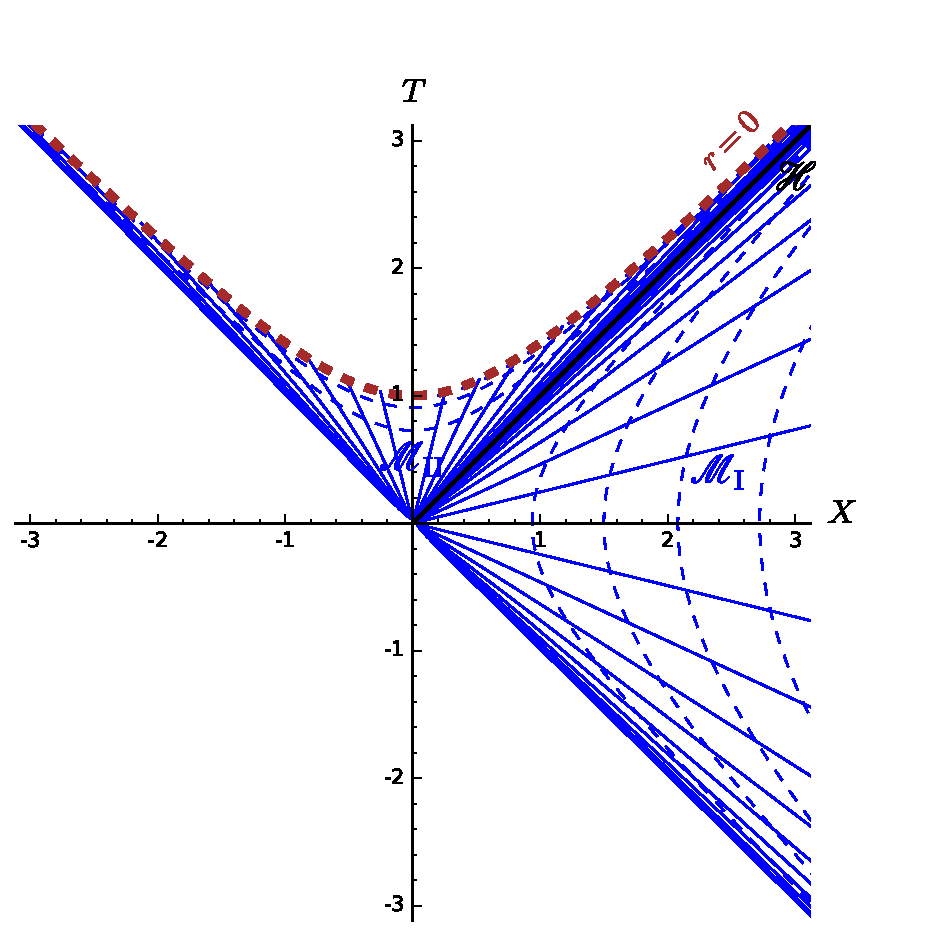
\includegraphics[width=0.6\textwidth]{sch_SD_KS.pdf}}
\caption[]{\label{f:sch:SD_KS} \footnotesize
Schwarzschild-Droste coordinates in $\M_{\rm SD} = \M_{\rm I}\cup \M_{\rm II}$
depicted in terms of the Kruskal-Szekeres coordinates $(T,X)$: the solid blue
curves have $t=\mathrm{const}$ (spaced apart by $\delta t = m$), while the
dashed blue curves have $r=\mathrm{const}$ (spaced apart by $\delta r = m/2$).}
\end{figure}


As discussed in Sec.~\ref{s:sch:singularities}, one approaches a
curvature singularity as $r\rightarrow 0$. According to (\ref{e:sch:KS_IEF})
or (\ref{e:sch:KS_SD_II}),
this corresponds to $X^2-T^2 \rightarrow -1$ (see also Fig.~\ref{f:sch:X2mT2}), with
$T > 0$. Hence, in the $(T,X)$ plane, the curvature singularity is located
at $T = \sqrt{X^2 + 1}$, i.e. at the upper branch of the hyperbola
$X^2 - T^2 = -1$.

\subsection{Radial null geodesics in Kruskal-Szekeres coordinates}

By construction, the Kruskal-Szekeres coordinates $(T,X,\th,\ph)$ are
adapted to the radial null geodesics. This is clear on the expression
(\ref{e:sch:metric_KS}) of the metric tensor, where the $(T,X)$ part is
conformal to the flat metric $- \D T^2 + \D X^2$. Consequently the radial
null geodesics are straight lines of slope $\pm 1$ in the $(T,X)$ plane
(cf. Fig.~\ref{f:sch:rad_null_geod_KS}):
\begin{itemize}
\item the ingoing radial null geodesics obey
\be
    T = - X + V ,
\ee
where $V$ is a positive constant (the constraint $V>0$ following from (\ref{e:sch:range_X_T_IEF})), so that each geodesic of this family can be labelled
by $(V,\th,\ph)$;
\item the outgoing radial null geodesics obey
\be \label{e:sch:outgoing_null_geod_KS}
    T = X + U ,
\ee
where $U$ is an arbitrary real constant, so that each geodesic of this family can be labelled
by $(U,\th,\ph)$.
\end{itemize}
\begin{figure}
\centerline{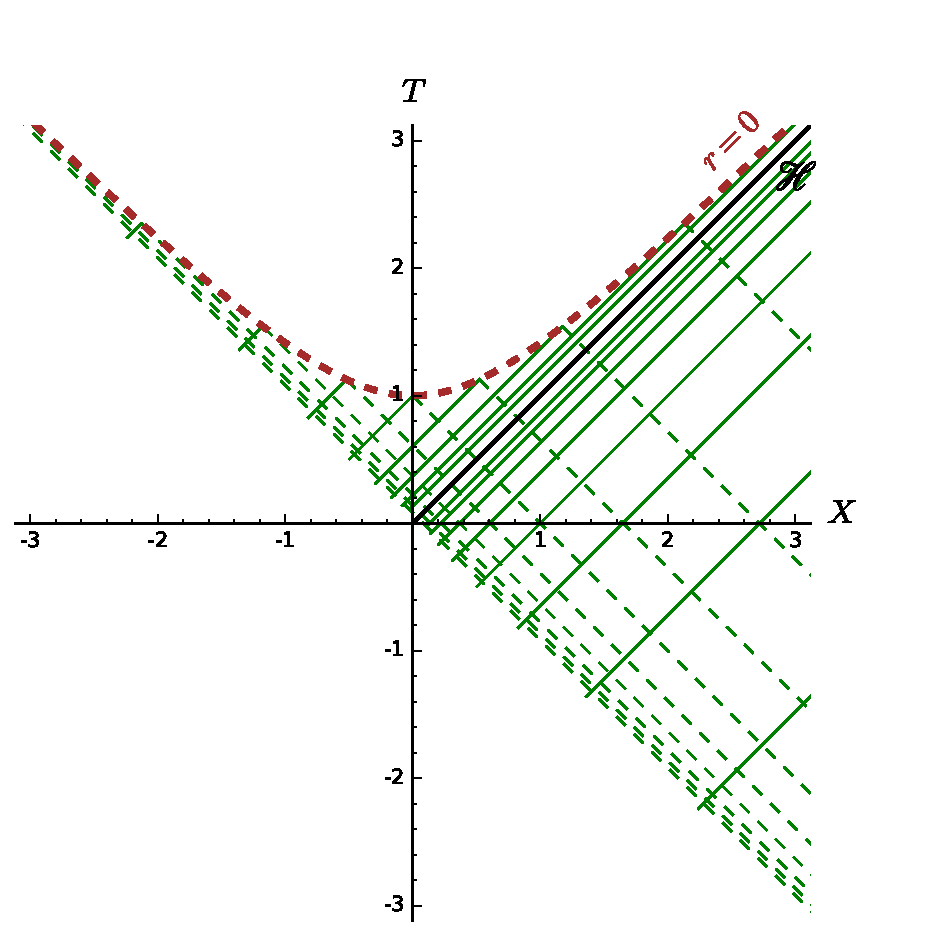
\includegraphics[width=0.6\textwidth]{sch_rad_null_geod_KS.pdf}}
\caption[]{\label{f:sch:rad_null_geod_KS} \footnotesize
Radial null geodesics in $\M_{\rm IEF} = \M_{\rm I}\cup\Hor\cup\M_{\rm II}$
depicted in terms of the Kruskal-Szekeres coordinates $(T,X)$: the solid
lines correspond to the outgoing family, with $u$ spanning $[-6m, 8m]$
(with steps $\delta u = 2m$), from the left to the right in $\M_{\rm II}$
and from the right to the left in $\M_{\rm I}$; the dashed lines
correspond to the ingoing family, with $v$ spanning $[-8m, 6m]$ (with steps $\delta v = 2m$)
from the left to the right.}
\end{figure}
In particular, the Schwarzschild horizon $\Hor$ is generated by the
outgoing radial null geodesics having $U=0$, as it clear from
(\ref{e:sch:outgoing_null_geod_KS}) and (\ref{e:sch:X2mT2}) that $U=0$
implies $r=2m$ for outgoing radial null geodesics.
The outgoing radial null geodesics not lying on $\Hor$ have an equation
in terms of the IEF coordinates given by
Eq.~(\ref{e:sch:outgoing_null_geod_EF}):
$\ti = r + 4 m \ln \left|r/2m- 1 \right| + u$,
where the constant $u$ is related to $U$ by
\begin{subequations}
\begin{align}
 & U = - \mathrm{e}^{-u/4m} \quad \mbox{on}\ \M_{\rm I} \\
 & U = 0 \quad \mbox{on}\ \Hor \\
 & U =  \mathrm{e}^{-u/4m} \quad \mbox{on}\ \M_{\rm II} .
\end{align}
\end{subequations}
These relations are easily established by combining
(\ref{e:sch:outgoing_null_geod_EF}) and (\ref{e:sch:KS_IEF}).


\begin{remark}
The relation $U = - \mathrm{e}^{-u/4m}$ introduced in Sec.~\ref{s:sch:KS_coord}
by Eq.~(\ref{e:sch:def_U_V}) is thus valid only in $\M_{\rm I}$. On the
contrary the relation $V = \mathrm{e}^{v/4m}$ is valid on all $\M_{\rm IEF}$.
\end{remark}

\subsection{Maximal extension}

The spacetime $(\M_{\rm IEF}, \w{g})$ is not geodesically complete.
Indeed, let us consider the radial null geodesics discussed above.
We have seen in Sec.~\ref{s:sch:rad_null_geod} that $r$ is an affine parameter
along them, except for those that are null generators of $\Hor$
(the outgoing ones with $U=0$).
Now, for the ingoing radial null geodesics, $r$ is decreasing towards the
future and all of them terminate at $r=0$ (cf. Fig.~\ref{f:sch:rad_null_geod_KS}).
They are thus incomplete geodesics. However, they cannot be extended to
negative values of the affine parameter $r$, since $r=0$ marks a
spacetime singularity (cf. Sec.~\ref{s:sch:singularities}).

On the other hand the outgoing radial null geodesics are limited by
the constraint $T+X > 0$, which corresponds to $r>2m$ in $\M_{\rm I}$, with $r$ increasing towards
the future, and to
$r<2m$ in $\M_{\rm II}$, with $r$ decreasing towards the future.
Thus all outgoing radial null geodesics terminate towards the past at the finite
value $2m$ of the affine parameter $r$
(cf. Fig.~\ref{f:sch:rad_null_geod_KS}) and are therefore incomplete geodesics.
However, contrary to ingoing radial null geodesics, they can be extended
since $r=2m$ does not mark a spacetime singularity.
More precisely, the limit at which outgoing radial null geodesics
terminate is $T=-X$, which by virtue of (\ref{e:sch:X2mT2}) yields $r=2m$.
This does not corresponds to the Schwarzschild horizon $\Hor$, since for
the latter $T=X$, but rather to $\ti\rightarrow-\infty$,
as it is clear when comparing Fig.~\ref{f:sch:rad_null_geod_KS}
with Fig.~\ref{f:sch:IEF_KS}.

The possibility of spacetime extension beyond $\M_{\rm IEF}$ is clear
on the metric element (\ref{e:sch:metric_KS_TX}): it is invariant by
the transformation $(T,X) \mapsto (-T,-X)$. Thus we may include
the part $T+X<0$ by adding a copy of $\M_{\rm IEF}$, symmetric to the
original one with respect to the ``origin'' $(T,X)=(0,0)$.
The whole spacetime manifold is then the following open subset of
$\R^2\times\mathbb{S}^2$:
\be
    \M = \{ p \in \R^2\times\mathbb{S}^2, \quad X^2(p) - T^2(p) > - 1 \} ,
\ee
where $(T,X,\th,\ph)$ is the canonical coordinate system on $\R^2\times\mathbb{S}^2$,
called in this context
\defin{Kruskal-Szekeres coordinates}\index{Kruskal-Szekeres!coordinates}.


\subsection{Bifurcate Killing horizon}


\begin{figure}
\centerline{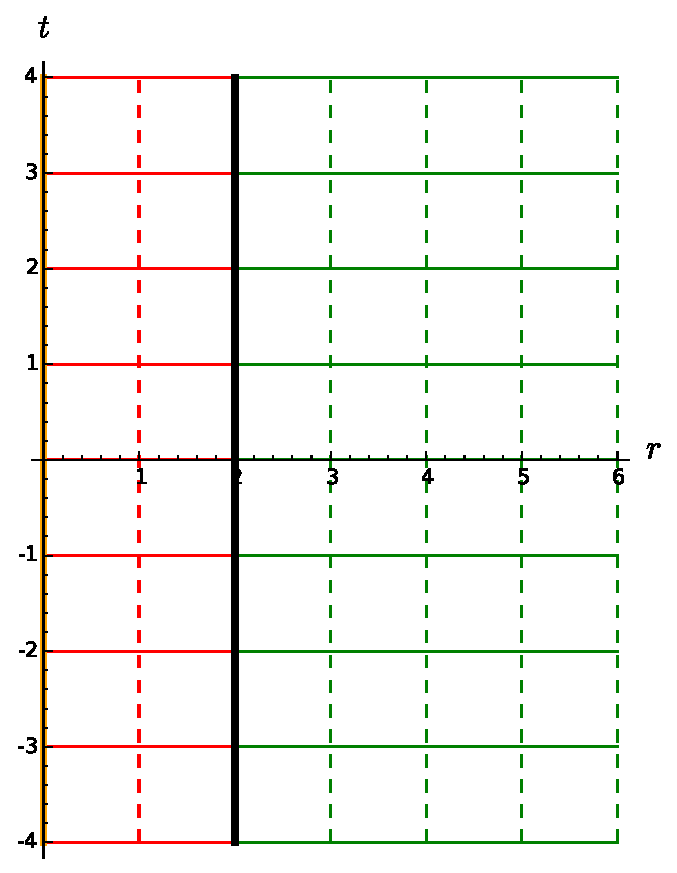
\includegraphics[height=0.37\textheight]{sch_coord_schwarz.pdf}\qquad
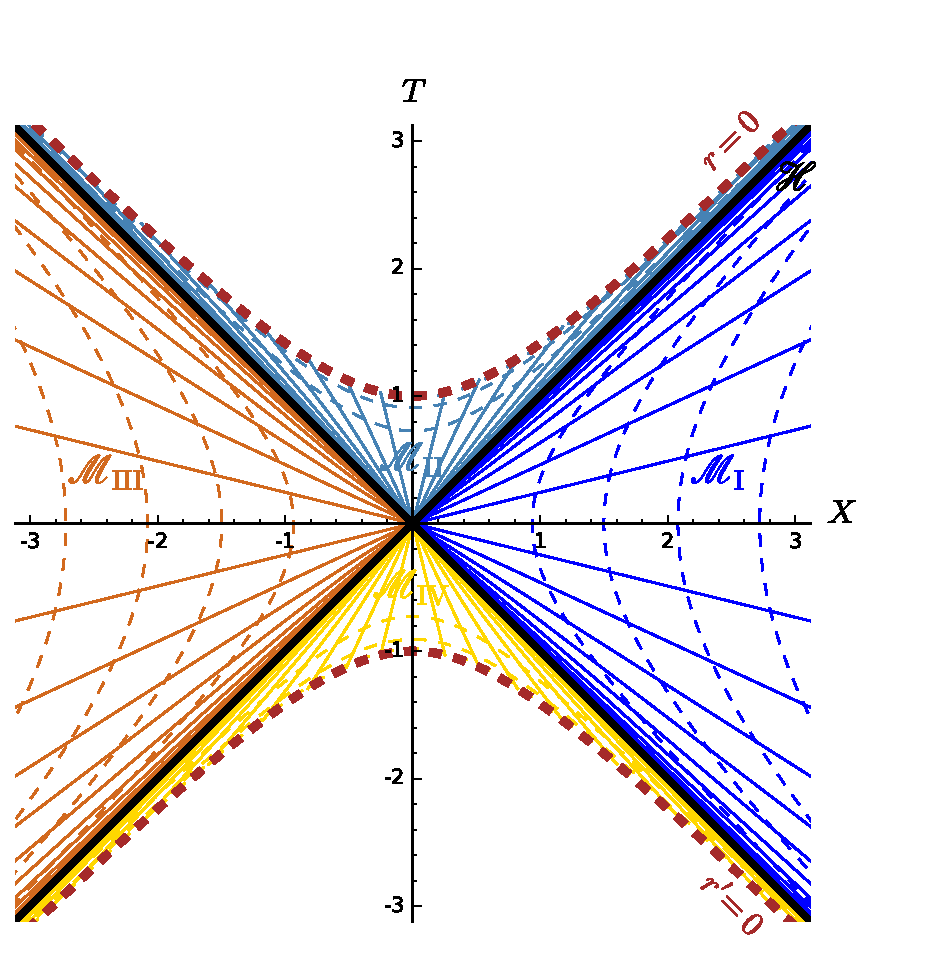
\includegraphics[height=0.37\textheight]{sch_kruskal_diag.pdf}}
\caption[]{\label{f:sch:kruskal_diag} \footnotesize
Schwarzschild spacetime depicted in Schwarzschild-Droste coordinates $(t,r)$
(left) and in Kruskal-Szekeres coordinates $(T,X)$ (right). In both figures,
green (resp. red) solid curves denote the hypersurfaces $t=\mathrm{const}$
in Region~I (resp. II), while green (resp. red) dashed curves
denote the hypersurfaces $r=\mathrm{const}$ in Region~I (resp. II).
The future and past event horizons are marked by thick black lines, while the
singularity at $r=0$ is depicted in orange. Regions III and IV are depicted
in grey and pink respectively. Note that the left figure covers only Regions I and II.}
\end{figure}

\begin{figure}
\centerline{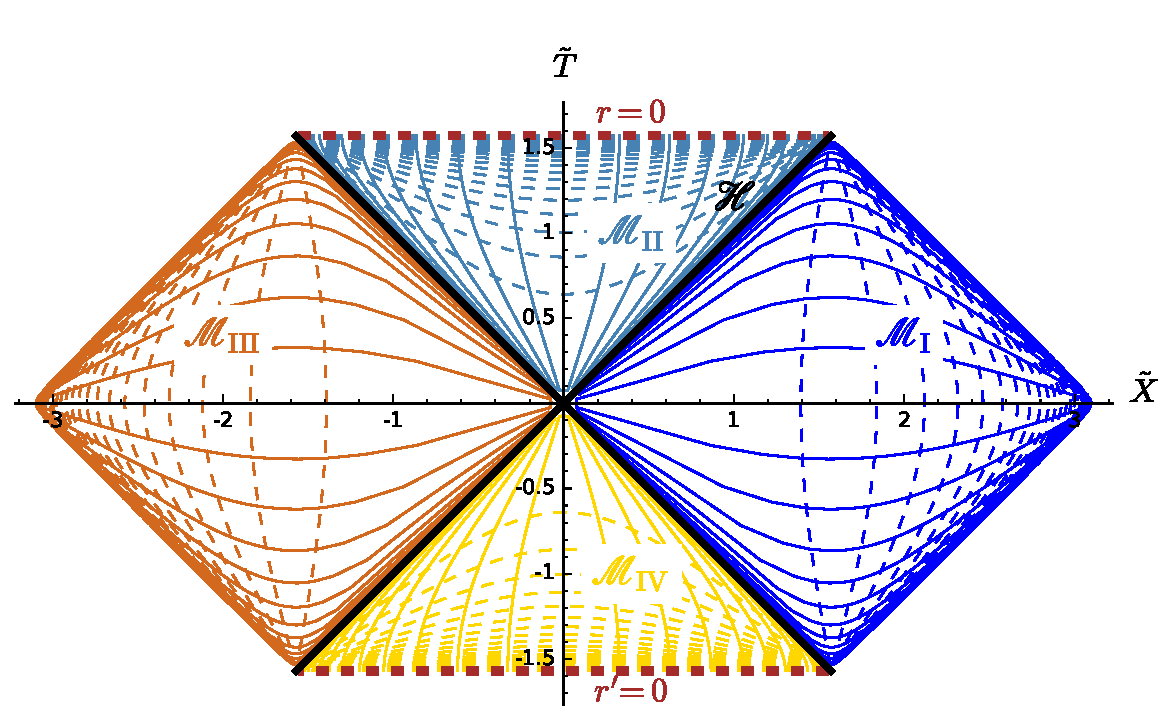
\includegraphics[width=0.9\textwidth]{sch_carter-penrose.pdf}}
\caption[]{\label{f:sch:sch_carter-penrose} \footnotesize
Schwarzschild spacetime depicted in Carter-Penrose coordinates $(\tilde{T},\tilde{X})$; the color code
is the same as in Fig.~\ref{f:sch:kruskal_diag}.
As Fig.~\ref{f:sch:kruskal_diag}, this figure has been produced with
SageManifolds (cf. Appendix~\ref{s:sam}).}
\end{figure}

